\vspace*{-2.0cm}
\textbf{\Huge LARGE SAMPLE HEADER}
\vspace{1.5cm}
\begin{tikzpicture}[remember picture,overlay]
   \node[anchor=south east,inner sep=20pt] at (current page.south east)
              {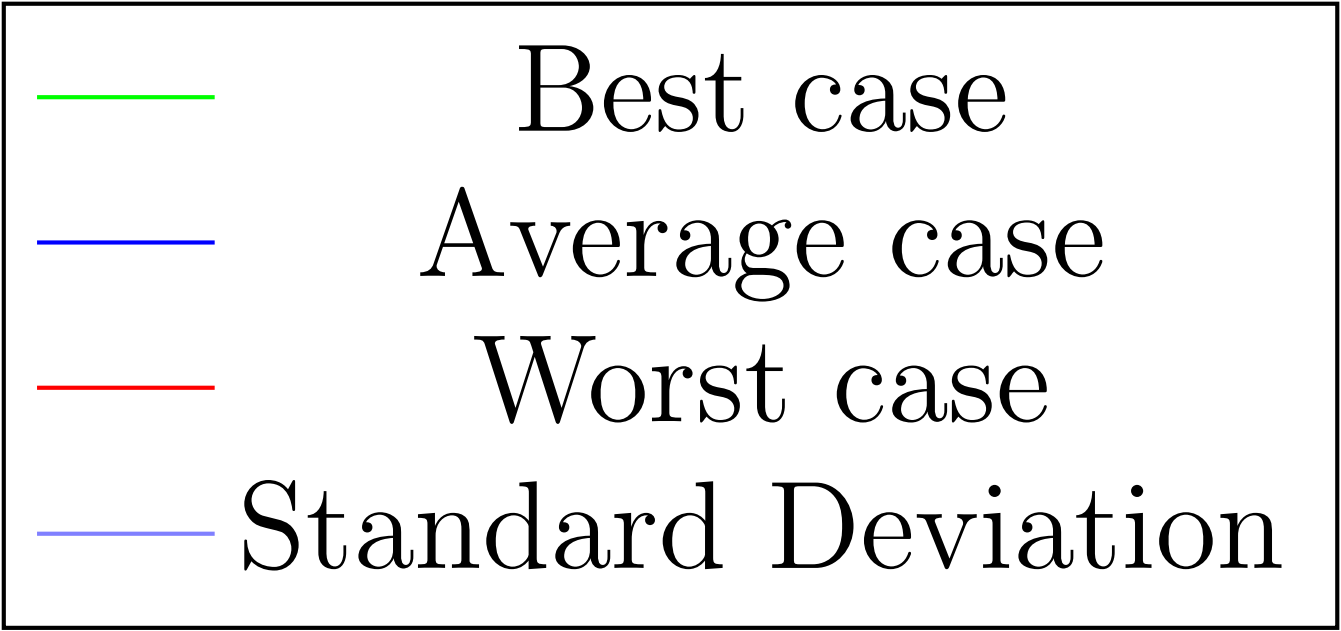
\includegraphics[scale=0.1]{chapters/res/generated_graph_legend.png}};
\end{tikzpicture}

\begin{figure}[H]
\vspace*{-1cm}
	\makebox[\linewidth][c]{%
	\begin{subfigure}[b]{0.7\textwidth}
		\centering
		\resizebox{0.9\linewidth}{!}{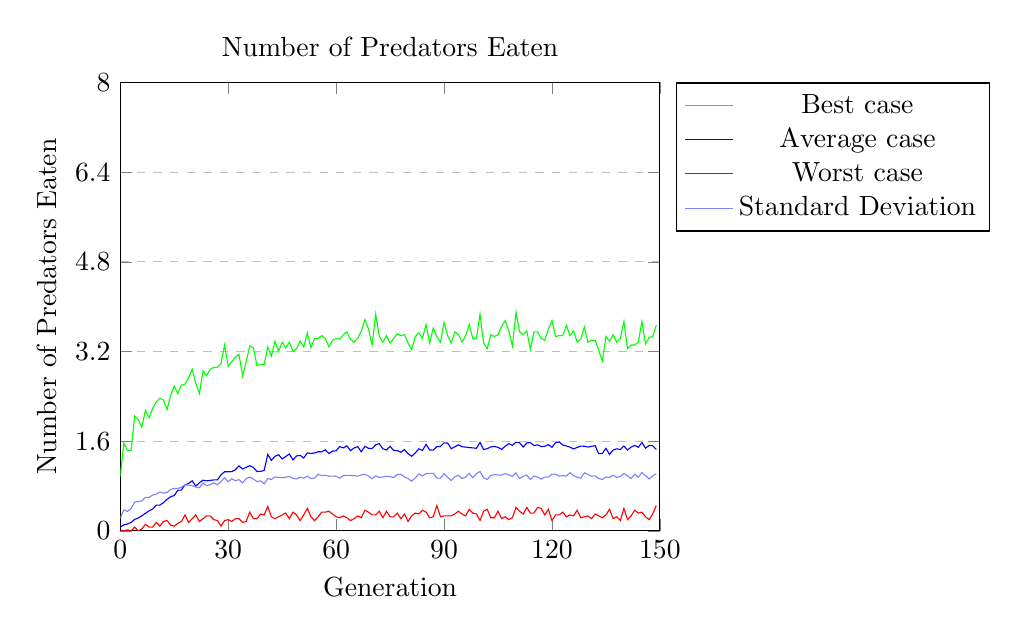
\begin{tikzpicture}
\begin{axis}[
	title={Number of Predators Eaten},
	xlabel={Generation},
	ylabel={Number of Predators Eaten},
	xmin=0, xmax=150,
	ymin=0, ymax=8,
	xtick={0.0,30.0,60.0,90.0,120.0,150.0},
	ytick={0.0,1.6,3.2,4.800000000000001,6.4,8.0},
	legend pos=outer north east,
	ymajorgrids=true,
	grid style=dashed,
]

\addplot[
	color=green,
	]
	coordinates {
	(0,0.9666666666666666)(1,1.5666666666666669)(2,1.4333333333333331)(3,1.4333333333333333)(4,2.05)(5,1.9833333333333336)(6,1.8500000000000003)(7,2.15)(8,2.016666666666667)(9,2.1833333333333336)(10,2.2999999999999994)(11,2.3666666666666676)(12,2.3333333333333335)(13,2.166666666666667)(14,2.416666666666667)(15,2.583333333333333)(16,2.4499999999999997)(17,2.6)(18,2.616666666666667)(19,2.7333333333333334)(20,2.8833333333333333)(21,2.6333333333333333)(22,2.4500000000000006)(23,2.85)(24,2.766666666666666)(25,2.8833333333333333)(26,2.916666666666667)(27,2.9166666666666665)(28,2.9833333333333325)(29,3.3166666666666664)(30,2.9333333333333327)(31,3.0166666666666666)(32,3.0999999999999996)(33,3.1499999999999995)(34,2.766666666666667)(35,3.0166666666666666)(36,3.3000000000000007)(37,3.2666666666666666)(38,2.9499999999999997)(39,2.966666666666667)(40,2.9666666666666663)(41,3.2833333333333328)(42,3.1166666666666667)(43,3.383333333333333)(44,3.2)(45,3.3666666666666663)(46,3.2666666666666666)(47,3.3666666666666667)(48,3.1999999999999997)(49,3.2499999999999996)(50,3.383333333333333)(51,3.2833333333333337)(52,3.533333333333333)(53,3.266666666666667)(54,3.433333333333333)(55,3.433333333333334)(56,3.483333333333333)(57,3.433333333333333)(58,3.283333333333333)(59,3.399999999999999)(60,3.4333333333333327)(61,3.4166666666666665)(62,3.5)(63,3.5500000000000003)(64,3.416666666666667)(65,3.366666666666667)(66,3.4333333333333336)(67,3.5666666666666664)(68,3.7666666666666666)(69,3.5999999999999996)(70,3.316666666666667)(71,3.8666666666666667)(72,3.466666666666666)(73,3.366666666666667)(74,3.4833333333333334)(75,3.349999999999999)(76,3.4333333333333345)(77,3.5166666666666657)(78,3.483333333333333)(79,3.5)(80,3.3500000000000005)(81,3.233333333333333)(82,3.466666666666667)(83,3.533333333333333)(84,3.4333333333333327)(85,3.6833333333333336)(86,3.3500000000000005)(87,3.6166666666666667)(88,3.4666666666666663)(89,3.3666666666666667)(90,3.716666666666667)(91,3.4833333333333334)(92,3.349999999999999)(93,3.549999999999999)(94,3.5)(95,3.366666666666667)(96,3.4833333333333325)(97,3.683333333333333)(98,3.4333333333333336)(99,3.4333333333333336)(100,3.8666666666666676)(101,3.3499999999999996)(102,3.2499999999999996)(103,3.5)(104,3.466666666666666)(105,3.4999999999999996)(106,3.650000000000001)(107,3.7499999999999996)(108,3.5666666666666664)(109,3.3)(110,3.9)(111,3.55)(112,3.5)(113,3.566666666666666)(114,3.2333333333333334)(115,3.55)(116,3.55)(117,3.433333333333333)(118,3.3999999999999995)(119,3.5999999999999996)(120,3.7499999999999996)(121,3.466666666666667)(122,3.483333333333333)(123,3.483333333333333)(124,3.6666666666666665)(125,3.4833333333333325)(126,3.5666666666666664)(127,3.3666666666666663)(128,3.416666666666667)(129,3.6333333333333333)(130,3.3666666666666663)(131,3.399999999999999)(132,3.3999999999999995)(133,3.216666666666667)(134,3.033333333333333)(135,3.4666666666666663)(136,3.383333333333333)(137,3.499999999999999)(138,3.3666666666666667)(139,3.433333333333334)(140,3.7333333333333334)(141,3.2500000000000004)(142,3.3166666666666664)(143,3.3166666666666673)(144,3.366666666666666)(145,3.733333333333333)(146,3.333333333333333)(147,3.45)(148,3.466666666666666)(149,3.6666666666666665)
	};
	\addlegendentry{Best case}
\addplot[
	color=blue,
	]
	coordinates {
	(0,0.06597222222222222)(1,0.10555555555555557)(2,0.12222222222222222)(3,0.14930555555555552)(4,0.2041666666666667)(5,0.2277777777777778)(6,0.2694444444444445)(7,0.31180555555555556)(8,0.35625)(9,0.38819444444444445)(10,0.4583333333333333)(11,0.4590277777777777)(12,0.5020833333333333)(13,0.5625000000000001)(14,0.6083333333333333)(15,0.6298611111111111)(16,0.7243055555555556)(17,0.7270833333333333)(18,0.8208333333333333)(19,0.8458333333333333)(20,0.8916666666666668)(21,0.7972222222222223)(22,0.8576388888888888)(23,0.9027777777777778)(24,0.8909722222222223)(25,0.8993055555555554)(26,0.9083333333333332)(27,0.9083333333333333)(28,1.0)(29,1.0534722222222221)(30,1.0541666666666667)(31,1.0555555555555556)(32,1.0909722222222222)(33,1.158333333333333)(34,1.1020833333333333)(35,1.1333333333333335)(36,1.1618055555555558)(37,1.1319444444444442)(38,1.0583333333333333)(39,1.0611111111111111)(40,1.0777777777777777)(41,1.363888888888889)(42,1.25625)(43,1.3291666666666664)(44,1.3590277777777777)(45,1.2826388888888889)(46,1.3256944444444447)(47,1.371527777777778)(48,1.2652777777777775)(49,1.3354166666666665)(50,1.3472222222222225)(51,1.298611111111111)(52,1.3902777777777777)(53,1.379861111111111)(54,1.3888888888888888)(55,1.4104166666666669)(56,1.409722222222222)(57,1.4451388888888888)(58,1.3791666666666667)(59,1.423611111111111)(60,1.4263888888888887)(61,1.5020833333333334)(62,1.4791666666666663)(63,1.5166666666666668)(64,1.430555555555556)(65,1.4777777777777776)(66,1.5020833333333334)(67,1.4111111111111114)(68,1.507638888888889)(69,1.472916666666667)(70,1.4666666666666668)(71,1.535416666666667)(72,1.5548611111111108)(73,1.4638888888888888)(74,1.4409722222222219)(75,1.5083333333333335)(76,1.4333333333333331)(77,1.4312499999999997)(78,1.402083333333333)(79,1.4500000000000002)(80,1.3763888888888889)(81,1.3305555555555555)(82,1.3888888888888884)(83,1.4631944444444447)(84,1.4340277777777777)(85,1.5416666666666665)(86,1.4437499999999999)(87,1.4388888888888893)(88,1.5013888888888887)(89,1.5048611111111112)(90,1.570138888888889)(91,1.5659722222222225)(92,1.4645833333333331)(93,1.4999999999999996)(94,1.5340277777777784)(95,1.5006944444444446)(96,1.49375)(97,1.4854166666666668)(98,1.479861111111111)(99,1.4729166666666667)(100,1.5777777777777777)(101,1.4493055555555556)(102,1.465972222222222)(103,1.498611111111111)(104,1.5055555555555555)(105,1.4888888888888892)(106,1.4541666666666668)(107,1.5090277777777776)(108,1.5555555555555558)(109,1.5243055555555558)(110,1.5798611111111107)(111,1.5715277777777774)(112,1.4958333333333333)(113,1.5701388888888888)(114,1.5743055555555556)(115,1.520833333333333)(116,1.5340277777777778)(117,1.503472222222222)(118,1.5083333333333333)(119,1.5381944444444444)(120,1.4902777777777776)(121,1.571527777777778)(122,1.5847222222222221)(123,1.5319444444444448)(124,1.5145833333333332)(125,1.4930555555555558)(126,1.4618055555555554)(127,1.4868055555555553)(128,1.5118055555555556)(129,1.5090277777777779)(130,1.4951388888888888)(131,1.5069444444444442)(132,1.5194444444444446)(133,1.3756944444444443)(134,1.3798611111111112)(135,1.4722222222222219)(136,1.3625)(137,1.4430555555555553)(138,1.4631944444444447)(139,1.4499999999999997)(140,1.5124999999999997)(141,1.4416666666666667)(142,1.4937500000000001)(143,1.5243055555555558)(144,1.4902777777777778)(145,1.5749999999999997)(146,1.4749999999999999)(147,1.522916666666667)(148,1.5180555555555555)(149,1.450694444444444)
	};
	\addlegendentry{Average case}
\addplot[
	color=red,
	]
	coordinates {
	(0,0.0)(1,0.0)(2,0.016666666666666666)(3,0.0)(4,0.06666666666666667)(5,0.0)(6,0.03333333333333333)(7,0.11666666666666667)(8,0.06666666666666667)(9,0.06666666666666667)(10,0.15)(11,0.08333333333333333)(12,0.16666666666666666)(13,0.18333333333333332)(14,0.1)(15,0.08333333333333333)(16,0.13333333333333333)(17,0.16666666666666666)(18,0.2833333333333333)(19,0.15)(20,0.21666666666666665)(21,0.2833333333333333)(22,0.16666666666666666)(23,0.21666666666666665)(24,0.26666666666666666)(25,0.26666666666666666)(26,0.19999999999999998)(27,0.18333333333333332)(28,0.08333333333333334)(29,0.18333333333333332)(30,0.19999999999999998)(31,0.16666666666666666)(32,0.21666666666666665)(33,0.21666666666666665)(34,0.15)(35,0.16666666666666666)(36,0.3333333333333333)(37,0.21666666666666665)(38,0.21666666666666665)(39,0.3)(40,0.2833333333333333)(41,0.4333333333333333)(42,0.24999999999999997)(43,0.21666666666666665)(44,0.24999999999999997)(45,0.2833333333333333)(46,0.31666666666666665)(47,0.21666666666666665)(48,0.3333333333333333)(49,0.2833333333333333)(50,0.18333333333333332)(51,0.2833333333333333)(52,0.39999999999999997)(53,0.24999999999999997)(54,0.18333333333333332)(55,0.24999999999999997)(56,0.3333333333333333)(57,0.3333333333333333)(58,0.35)(59,0.3)(60,0.24999999999999997)(61,0.2333333333333333)(62,0.26666666666666666)(63,0.2333333333333333)(64,0.18333333333333332)(65,0.21666666666666665)(66,0.26666666666666666)(67,0.2333333333333333)(68,0.36666666666666664)(69,0.3333333333333333)(70,0.2833333333333333)(71,0.2833333333333333)(72,0.35)(73,0.2333333333333333)(74,0.35)(75,0.24999999999999997)(76,0.24999999999999997)(77,0.31666666666666665)(78,0.21666666666666665)(79,0.3)(80,0.16666666666666666)(81,0.26666666666666666)(82,0.31666666666666665)(83,0.3)(84,0.36666666666666664)(85,0.3333333333333333)(86,0.2333333333333333)(87,0.24999999999999997)(88,0.44999999999999996)(89,0.24999999999999997)(90,0.26666666666666666)(91,0.26666666666666666)(92,0.26666666666666666)(93,0.3)(94,0.35)(95,0.3)(96,0.26666666666666666)(97,0.3833333333333333)(98,0.31666666666666665)(99,0.3)(100,0.18333333333333332)(101,0.35)(102,0.3833333333333333)(103,0.2333333333333333)(104,0.2333333333333333)(105,0.35)(106,0.21666666666666665)(107,0.24999999999999997)(108,0.19999999999999998)(109,0.2333333333333333)(110,0.41666666666666663)(111,0.35)(112,0.3)(113,0.41666666666666663)(114,0.31666666666666665)(115,0.31666666666666665)(116,0.41666666666666663)(117,0.39999999999999997)(118,0.2833333333333333)(119,0.3833333333333333)(120,0.18333333333333332)(121,0.2833333333333333)(122,0.2833333333333333)(123,0.3333333333333333)(124,0.24999999999999997)(125,0.2833333333333333)(126,0.26666666666666666)(127,0.36666666666666664)(128,0.2333333333333333)(129,0.24999999999999997)(130,0.26666666666666666)(131,0.21666666666666665)(132,0.3)(133,0.26666666666666666)(134,0.2333333333333333)(135,0.2833333333333333)(136,0.3833333333333333)(137,0.21666666666666665)(138,0.24999999999999997)(139,0.18333333333333332)(140,0.39999999999999997)(141,0.19999999999999998)(142,0.26666666666666666)(143,0.36666666666666664)(144,0.31666666666666665)(145,0.3333333333333333)(146,0.24999999999999997)(147,0.19999999999999998)(148,0.3)(149,0.44999999999999996)
	};
	\addlegendentry{Worst case}
\addplot[
	color=blue!50,
	]
	coordinates {
	(0,0.22810186512317995)(1,0.3718097332768811)(2,0.345647402635599)(3,0.39699357623545967)(4,0.5138792555180911)(5,0.5206370865039666)(6,0.5354322880656994)(7,0.5959918288673569)(8,0.5957464980983094)(9,0.6381545461207714)(10,0.6544157192161484)(11,0.6927992034441525)(12,0.6722084507491709)(13,0.6843365883572965)(14,0.7384416963839964)(15,0.7553805146012672)(16,0.7567879875086504)(17,0.7761000580438222)(18,0.8239608598665922)(19,0.8141765811345567)(20,0.8059054603391009)(21,0.7827695395066535)(22,0.7685798512811592)(23,0.8545075912627764)(24,0.8066600194512461)(25,0.8213047161793012)(26,0.8566928186325042)(27,0.8219235106348346)(28,0.8818150722779325)(29,0.9483172788083861)(30,0.8759037593822429)(31,0.928085110238431)(32,0.8933512538685642)(33,0.9145676016751958)(34,0.8540885600591401)(35,0.9361875717102862)(36,0.9532635109306814)(37,0.9248288480881136)(38,0.8780358726506764)(39,0.8920947846161121)(40,0.8389079397070467)(41,0.9310517560644359)(42,0.9169672329669347)(43,0.9626393230017223)(44,0.953305984898185)(45,0.9475155563329191)(46,0.9563120633890103)(47,0.9690109120939004)(48,0.9370607511828415)(49,0.9251085904346795)(50,0.9593348140607003)(51,0.9388820833026523)(52,0.9772060224313383)(53,0.9327708529184457)(54,0.9412102328931546)(55,1.0077411580389004)(56,0.9852037990060252)(57,0.9911527973635053)(58,0.9739897240274592)(59,0.9762958851755198)(60,0.9728815797212503)(61,0.9397801191846543)(62,0.9860176940119886)(63,0.9887585575026453)(64,0.9878949236675736)(65,0.9857002506497867)(66,0.9742204622105117)(67,0.997738909615304)(68,1.0070425414875266)(69,0.977663045346536)(70,0.928886568602237)(71,0.9791505985330582)(72,0.9545986319347426)(73,0.9616850879978396)(74,0.9732365499001447)(75,0.9646654709337494)(76,0.9508629094932712)(77,1.0025603129489447)(78,1.0095566600655457)(79,0.9595891281644218)(80,0.9337702023850106)(81,0.8861973519209494)(82,0.9433294526574671)(83,1.0152919365875552)(84,0.9787093157423733)(85,1.0222555976967989)(86,1.0247018937565666)(87,1.0262721417066973)(88,0.9412691816448212)(89,0.9407486267702396)(90,1.0194751751230433)(91,0.955970674775724)(92,0.8982605274530155)(93,0.9641212560889841)(94,0.9929408862575011)(95,0.9337221659166333)(96,0.9572120942865925)(97,1.0259309967342551)(98,0.9501115634388491)(99,1.019286121940842)(100,1.0586653743886223)(101,0.944150328954389)(102,0.9165038721252468)(103,0.9882369427730343)(104,1.0024095780547078)(105,0.997845039428861)(106,0.9929675230837386)(107,1.0209746253543222)(108,0.9964515312484529)(109,0.9732781796446134)(110,1.0326336414888901)(111,0.9319156849314015)(112,0.9716152138162422)(113,0.9957941705810749)(114,0.9173588293084006)(115,0.9782184152846188)(116,0.9597984307842808)(117,0.9224617398001695)(118,0.9582514881452882)(119,0.958707393381238)(120,1.0129407727703712)(121,1.009816594443192)(122,0.9762712582599299)(123,0.9847047252553303)(124,0.977086094849565)(125,1.0368969148123457)(126,0.9844155409431966)(127,0.9564477843400175)(128,0.9369375197935595)(129,1.0356988710778785)(130,1.006687832266945)(131,0.9736212916755186)(132,0.9818050306273509)(133,0.9314510779420476)(134,0.9174090582062905)(135,0.9607146057643011)(136,0.9477226927053267)(137,0.9946920048277378)(138,0.9529447551456616)(139,0.9707813834396313)(140,1.021358396528527)(141,0.9813965194540895)(142,0.9343798771309901)(143,1.009943885726864)(144,0.9544205477403176)(145,1.042712213375269)(146,0.9850693099959399)(147,0.9250773473950887)(148,0.981919924129806)(149,1.0147175457773097)
	};
	\addlegendentry{Standard Deviation}
\end{axis}
\end{tikzpicture}
}
		\caption{Some sample caption}
	\end{subfigure}%
	\begin{subfigure}[b]{0.7\textwidth}	
		\centering
		\resizebox{0.9\linewidth}{!}{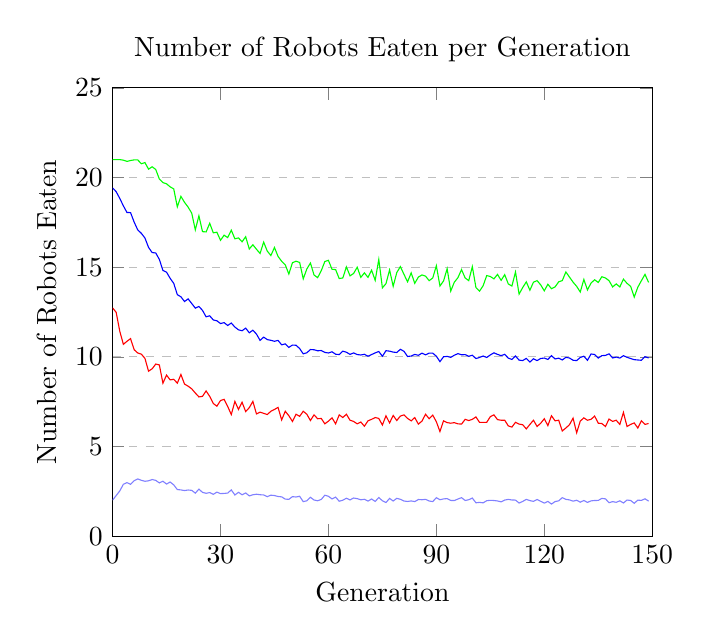
\begin{tikzpicture}
\begin{axis}[
	title={Number of Robots Eaten per Generation},
	xlabel={Generation},
	ylabel={Number of Robots Eaten},
	xmin=0, xmax=150,
	ymin=0, ymax=25,
	xtick={0.0,30.0,60.0,90.0,120.0,150.0},
	ytick={0.0,5.0,10.0,15.0,20.0,25.0},
	ymajorgrids=true,
	grid style=dashed,
]

\addplot[
	color=green,
	]
	coordinates {
	(0,21.000000000000007)(1,21.000000000000007)(2,21.000000000000007)(3,20.966666666666672)(4,20.900000000000006)(5,20.950000000000006)(6,20.98333333333334)(7,20.98333333333334)(8,20.766666666666673)(9,20.83333333333334)(10,20.466666666666672)(11,20.600000000000005)(12,20.450000000000003)(13,19.91666666666667)(14,19.716666666666672)(15,19.650000000000006)(16,19.483333333333338)(17,19.366666666666667)(18,18.366666666666667)(19,18.950000000000003)(20,18.61666666666667)(21,18.349999999999998)(22,18.016666666666666)(23,17.083333333333332)(24,17.866666666666664)(25,16.983333333333327)(26,16.96666666666667)(27,17.45)(28,16.916666666666664)(29,16.95)(30,16.5)(31,16.78333333333333)(32,16.649999999999995)(33,17.066666666666666)(34,16.583333333333332)(35,16.633333333333336)(36,16.416666666666664)(37,16.7)(38,16.016666666666666)(39,16.25)(40,16.0)(41,15.766666666666664)(42,16.4)(43,15.899999999999997)(44,15.649999999999999)(45,16.1)(46,15.600000000000001)(47,15.333333333333332)(48,15.133333333333335)(49,14.616666666666664)(50,15.25)(51,15.333333333333334)(52,15.266666666666666)(53,14.349999999999998)(54,14.900000000000002)(55,15.233333333333333)(56,14.566666666666665)(57,14.416666666666668)(58,14.8)(59,15.316666666666668)(60,15.383333333333331)(61,14.883333333333333)(62,14.866666666666665)(63,14.366666666666667)(64,14.399999999999999)(65,15.016666666666664)(66,14.516666666666667)(67,14.649999999999997)(68,14.999999999999998)(69,14.433333333333334)(70,14.683333333333332)(71,14.433333333333332)(72,14.833333333333332)(73,14.266666666666667)(74,15.433333333333332)(75,13.850000000000001)(76,14.083333333333332)(77,14.849999999999998)(78,13.933333333333334)(79,14.699999999999998)(80,15.033333333333333)(81,14.600000000000001)(82,14.183333333333334)(83,14.683333333333334)(84,14.100000000000001)(85,14.450000000000001)(86,14.566666666666663)(87,14.5)(88,14.250000000000002)(89,14.4)(90,15.083333333333334)(91,13.950000000000001)(92,14.233333333333333)(93,14.916666666666664)(94,13.666666666666671)(95,14.166666666666663)(96,14.416666666666668)(97,14.866666666666665)(98,14.4)(99,14.25)(100,15.033333333333333)(101,13.866666666666664)(102,13.66666666666667)(103,13.966666666666665)(104,14.533333333333333)(105,14.483333333333334)(106,14.350000000000001)(107,14.600000000000001)(108,14.26666666666667)(109,14.583333333333332)(110,14.066666666666666)(111,13.95)(112,14.733333333333334)(113,13.499999999999998)(114,13.866666666666665)(115,14.183333333333334)(116,13.716666666666669)(117,14.166666666666666)(118,14.249999999999998)(119,14.016666666666667)(120,13.683333333333332)(121,14.05)(122,13.8)(123,13.899999999999999)(124,14.183333333333334)(125,14.25)(126,14.733333333333336)(127,14.450000000000003)(128,14.166666666666664)(129,13.933333333333332)(130,13.616666666666665)(131,14.316666666666666)(132,13.733333333333333)(133,14.116666666666665)(134,14.299999999999999)(135,14.15)(136,14.46666666666667)(137,14.400000000000004)(138,14.250000000000002)(139,13.9)(140,14.066666666666668)(141,13.899999999999999)(142,14.333333333333332)(143,14.100000000000001)(144,13.933333333333334)(145,13.333333333333336)(146,13.883333333333333)(147,14.249999999999998)(148,14.6)(149,14.150000000000002)
	};
\addplot[
	color=blue,
	]
	coordinates {
	(0,19.422916666666666)(1,19.211111111111116)(2,18.837500000000002)(3,18.42291666666667)(4,18.050694444444446)(5,18.045833333333338)(6,17.51319444444444)(7,17.07986111111111)(8,16.889583333333338)(9,16.62708333333333)(10,16.105555555555554)(11,15.81736111111111)(12,15.792361111111113)(13,15.43611111111111)(14,14.817361111111111)(15,14.725000000000001)(16,14.38055555555556)(17,14.099999999999998)(18,13.46875)(19,13.349305555555556)(20,13.087500000000004)(21,13.231944444444446)(22,12.977083333333335)(23,12.718055555555559)(24,12.81111111111111)(25,12.592361111111112)(26,12.23263888888889)(27,12.290972222222223)(28,12.05833333333333)(29,12.011805555555558)(30,11.858333333333336)(31,11.909027777777778)(32,11.749999999999998)(33,11.886805555555554)(34,11.661805555555556)(35,11.508333333333335)(36,11.455555555555554)(37,11.602777777777776)(38,11.34375)(39,11.48611111111111)(40,11.271527777777775)(41,10.918750000000003)(42,11.100694444444445)(43,10.963194444444445)(44,10.922916666666667)(45,10.869444444444445)(46,10.91875)(47,10.670138888888888)(48,10.726388888888886)(49,10.528472222222222)(50,10.658333333333333)(51,10.64722222222222)(52,10.465277777777779)(53,10.16875)(54,10.22847222222222)(55,10.408333333333335)(56,10.397222222222222)(57,10.338888888888892)(58,10.354861111111111)(59,10.249305555555555)(60,10.216666666666667)(61,10.283333333333335)(62,10.147222222222222)(63,10.128472222222221)(64,10.318055555555555)(65,10.257638888888888)(66,10.13888888888889)(67,10.220833333333333)(68,10.129166666666666)(69,10.104166666666668)(70,10.143749999999999)(71,10.035416666666668)(72,10.130555555555556)(73,10.220833333333335)(74,10.299999999999997)(75,10.034027777777778)(76,10.343055555555555)(77,10.319444444444445)(78,10.264583333333333)(79,10.244444444444445)(80,10.420833333333334)(81,10.310416666666669)(82,10.022222222222222)(83,10.045138888888888)(84,10.136805555555556)(85,10.086111111111112)(86,10.20625)(87,10.113194444444446)(88,10.20833333333333)(89,10.206249999999999)(90,10.037499999999998)(91,9.734027777777778)(92,10.005555555555555)(93,10.027083333333334)(94,9.971527777777778)(95,10.093055555555557)(96,10.180555555555557)(97,10.113194444444444)(98,10.127083333333335)(99,10.033333333333333)(100,10.090972222222218)(101,9.904166666666667)(102,9.968055555555555)(103,10.047222222222224)(104,9.965972222222224)(105,10.107638888888888)(106,10.22638888888889)(107,10.137499999999998)(108,10.068750000000001)(109,10.140972222222224)(110,9.929861111111112)(111,9.855555555555556)(112,10.04722222222222)(113,9.81736111111111)(114,9.792361111111111)(115,9.915277777777778)(116,9.709722222222222)(117,9.894444444444444)(118,9.792361111111113)(119,9.910416666666665)(120,9.934027777777777)(121,9.856250000000001)(122,10.068055555555555)(123,9.882638888888888)(124,9.929166666666667)(125,9.827083333333333)(126,9.973611111111111)(127,9.936805555555557)(128,9.811111111111112)(129,9.793055555555554)(130,9.96597222222222)(131,10.036805555555555)(132,9.808333333333334)(133,10.162499999999998)(134,10.129861111111111)(135,9.933333333333332)(136,10.06875)(137,10.080555555555556)(138,10.16875)(139,9.939583333333333)(140,9.9875)(141,9.933333333333334)(142,10.068055555555555)(143,9.975000000000001)(144,9.90763888888889)(145,9.84375)(146,9.825694444444446)(147,9.810416666666669)(148,10.009722222222223)(149,9.938888888888888)
	};
\addplot[
	color=red,
	]
	coordinates {
	(0,12.733333333333336)(1,12.483333333333334)(2,11.433333333333334)(3,10.700000000000001)(4,10.866666666666667)(5,11.016666666666667)(6,10.400000000000002)(7,10.216666666666667)(8,10.149999999999999)(9,9.916666666666664)(10,9.200000000000003)(11,9.333333333333336)(12,9.600000000000001)(13,9.55)(14,8.533333333333335)(15,8.983333333333334)(16,8.716666666666667)(17,8.75)(18,8.533333333333333)(19,9.016666666666667)(20,8.483333333333333)(21,8.366666666666667)(22,8.216666666666667)(23,7.9833333333333325)(24,7.7666666666666675)(25,7.799999999999998)(26,8.1)(27,7.799999999999999)(28,7.399999999999998)(29,7.25)(30,7.566666666666668)(31,7.633333333333333)(32,7.233333333333333)(33,6.783333333333332)(34,7.516666666666668)(35,7.0666666666666655)(36,7.466666666666668)(37,6.949999999999999)(38,7.166666666666666)(39,7.516666666666667)(40,6.8166666666666655)(41,6.916666666666665)(42,6.8500000000000005)(43,6.783333333333335)(44,6.966666666666666)(45,7.066666666666667)(46,7.183333333333334)(47,6.483333333333332)(48,6.966666666666666)(49,6.716666666666666)(50,6.4)(51,6.8)(52,6.683333333333334)(53,6.966666666666666)(54,6.800000000000001)(55,6.4499999999999975)(56,6.766666666666666)(57,6.55)(58,6.566666666666666)(59,6.266666666666666)(60,6.416666666666666)(61,6.6)(62,6.266666666666666)(63,6.766666666666667)(64,6.616666666666666)(65,6.8)(66,6.466666666666666)(67,6.4)(68,6.266666666666666)(69,6.366666666666667)(70,6.133333333333335)(71,6.433333333333333)(72,6.5166666666666675)(73,6.616666666666666)(74,6.5666666666666655)(75,6.199999999999999)(76,6.716666666666669)(77,6.316666666666666)(78,6.7333333333333325)(79,6.449999999999998)(80,6.7)(81,6.766666666666667)(82,6.566666666666666)(83,6.433333333333334)(84,6.616666666666667)(85,6.250000000000001)(86,6.416666666666666)(87,6.8)(88,6.549999999999999)(89,6.749999999999998)(90,6.383333333333335)(91,5.833333333333333)(92,6.433333333333334)(93,6.333333333333332)(94,6.3)(95,6.333333333333333)(96,6.266666666666666)(97,6.249999999999999)(98,6.516666666666666)(99,6.449999999999999)(100,6.516666666666667)(101,6.6499999999999995)(102,6.3500000000000005)(103,6.35)(104,6.349999999999999)(105,6.666666666666666)(106,6.766666666666667)(107,6.499999999999999)(108,6.466666666666667)(109,6.466666666666666)(110,6.149999999999999)(111,6.083333333333334)(112,6.35)(113,6.250000000000001)(114,6.216666666666668)(115,5.983333333333333)(116,6.2333333333333325)(117,6.466666666666667)(118,6.116666666666668)(119,6.300000000000001)(120,6.55)(121,6.166666666666668)(122,6.716666666666665)(123,6.433333333333333)(124,6.466666666666667)(125,5.866666666666667)(126,6.033333333333333)(127,6.216666666666667)(128,6.583333333333333)(129,5.766666666666666)(130,6.416666666666666)(131,6.6)(132,6.466666666666666)(133,6.516666666666666)(134,6.699999999999999)(135,6.3)(136,6.283333333333334)(137,6.116666666666666)(138,6.533333333333332)(139,6.3999999999999995)(140,6.466666666666665)(141,6.233333333333333)(142,6.8999999999999995)(143,6.116666666666665)(144,6.2333333333333325)(145,6.316666666666666)(146,6.033333333333333)(147,6.433333333333334)(148,6.2333333333333325)(149,6.283333333333334)
	};
\addplot[
	color=blue!50,
	]
	coordinates {
	(0,2.0113996005838635)(1,2.2655504562278455)(2,2.523428127338372)(3,2.893897423121901)(4,2.9871822928142326)(5,2.8918968080680627)(6,3.096152416787628)(7,3.1947663840800775)(8,3.116582184803458)(9,3.0625628948276606)(10,3.088398573928132)(11,3.1601776571620803)(12,3.11341262394878)(13,2.971398344151116)(14,3.06614123565838)(15,2.9060661139400845)(16,3.021158320712189)(17,2.861439826087297)(18,2.6003656040557708)(19,2.5806621327374137)(20,2.5448185766978018)(21,2.574726725943908)(22,2.5578593675944723)(23,2.40115494497435)(24,2.6247028738208273)(25,2.443123536140499)(26,2.3929554749092263)(27,2.431079502448026)(28,2.3358855371024196)(29,2.455976942365564)(30,2.375087540335267)(31,2.384771373914672)(32,2.404685694641398)(33,2.5816980161392284)(34,2.297047689823935)(35,2.4485912083596513)(36,2.3098481664582846)(37,2.41149041509496)(38,2.2471607125399964)(39,2.308838414195794)(40,2.341908447385709)(41,2.312535325828631)(42,2.298721389611761)(43,2.205061751636127)(44,2.2875895143938827)(45,2.266955033185302)(46,2.2139667780639236)(47,2.1935510635671744)(48,2.0687648634365234)(49,2.0545686330476727)(50,2.2055585186985605)(51,2.1850688892750294)(52,2.2269862286438173)(53,1.9264278418564131)(54,1.9738967352367478)(55,2.1690059870394753)(56,2.0173523025563607)(57,1.9767057087670006)(58,2.049017498246475)(59,2.285754671814331)(60,2.225965931591818)(61,2.0781486159288383)(62,2.178753197459309)(63,1.9483248658673213)(64,2.0077682344840406)(65,2.116536805925538)(66,2.0241064392397696)(67,2.128581489300377)(68,2.0936853665373265)(69,2.028433424718565)(70,2.056973610743671)(71,1.9568840865375499)(72,2.0762553542894326)(73,1.9379167376002602)(74,2.156396583454864)(75,1.974947342812672)(76,1.8791106317170232)(77,2.107867209533473)(78,1.9627413337381523)(79,2.1117674474423227)(80,2.0573151374234526)(81,1.962497890883103)(82,1.9370373765350182)(83,1.9651318768331705)(84,1.9309095516477237)(85,2.0455965865726524)(86,2.0335901945053156)(87,2.0553178281795685)(88,1.9630050391005152)(89,1.929738818337511)(90,2.1475524139172415)(91,2.032266524353691)(92,2.079539681480517)(93,2.096309181288721)(94,1.994101735474168)(95,1.9885174942042725)(96,2.072921590049966)(97,2.1491137043758153)(98,1.991836421647755)(99,2.0327704181702075)(100,2.127009120922501)(101,1.8627280658001233)(102,1.8843106883309968)(103,1.8600047687719843)(104,1.9781530489036958)(105,2.0004393939225618)(106,1.9905902184375726)(107,1.9650315763564947)(108,1.9162297980300185)(109,2.01450144528217)(110,2.0536696301117803)(111,2.018536108751344)(112,2.0141474454495207)(113,1.8483255759174422)(114,1.9378582863595812)(115,2.05349579201371)(116,1.9845712197978036)(117,1.9407422354604016)(118,2.048149155491315)(119,1.943493054279464)(120,1.845400689140209)(121,1.939649979266822)(122,1.7928649191375787)(123,1.929929208687165)(124,1.9714707615015763)(125,2.148818763612173)(126,2.054244734087596)(127,2.0251514333575074)(128,1.9530007698209328)(129,2.0028252223945135)(130,1.8980163699486958)(131,1.9903199966926706)(132,1.8843253066567944)(133,1.969885674032518)(134,1.991229157137803)(135,1.9944395098710415)(136,2.1089209643957108)(137,2.0818808510389504)(138,1.868140827387872)(139,1.9269487312153624)(140,1.888974106705156)(141,1.9719484911636793)(142,1.850660754242215)(143,2.0158816949093867)(144,1.9931779658014623)(145,1.8352893878127157)(146,2.009082649009219)(147,1.996841607573629)(148,2.085186695851752)(149,1.956308451005405)
	};
\end{axis}
\end{tikzpicture}
}
		\caption{Some sample caption}
	\end{subfigure}%
}
\\
\\
\\
	\makebox[\linewidth][c]{%
	\begin{subfigure}[b]{0.7\textwidth}
		\centering
		\resizebox{0.9\linewidth}{!}{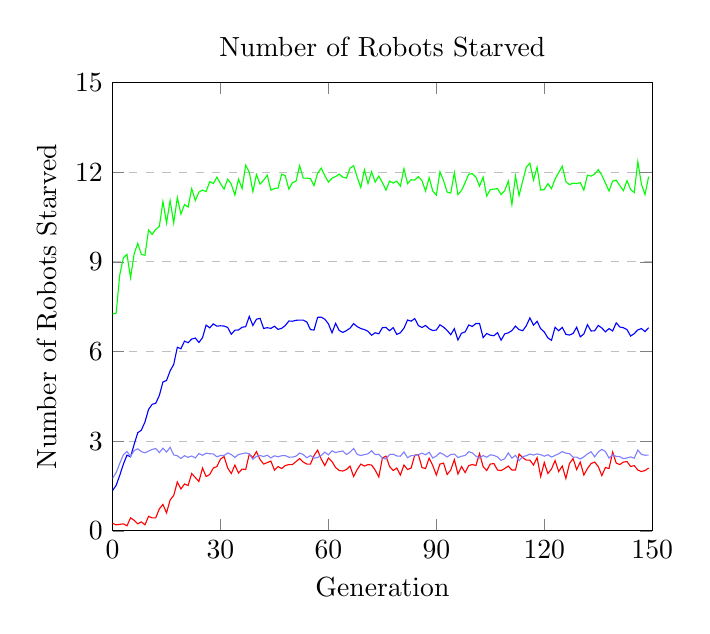
\begin{tikzpicture}
\begin{axis}[
	title={Number of Robots Starved},
	xlabel={Generation},
	ylabel={Number of Robots Starved},
	xmin=0, xmax=150,
	ymin=0, ymax=15,
	xtick={0.0,30.0,60.0,90.0,120.0,150.0},
	ytick={0.0,3.0,6.0,9.0,12.0,15.0},
	ymajorgrids=true,
	grid style=dashed,
]

\addplot[
	color=green,
	]
	coordinates {
	(0,7.250000000000002)(1,7.283333333333334)(2,8.566666666666668)(3,9.133333333333331)(4,9.25)(5,8.466666666666667)(6,9.266666666666667)(7,9.616666666666665)(8,9.25)(9,9.216666666666665)(10,10.066666666666666)(11,9.916666666666668)(12,10.083333333333332)(13,10.183333333333334)(14,11.01666666666667)(15,10.3)(16,11.050000000000002)(17,10.3)(18,11.15)(19,10.600000000000001)(20,10.916666666666666)(21,10.833333333333336)(22,11.450000000000003)(23,11.049999999999999)(24,11.333333333333332)(25,11.399999999999999)(26,11.349999999999998)(27,11.683333333333334)(28,11.616666666666667)(29,11.833333333333334)(30,11.616666666666669)(31,11.433333333333335)(32,11.766666666666666)(33,11.599999999999998)(34,11.233333333333334)(35,11.766666666666667)(36,11.450000000000001)(37,12.233333333333334)(38,12.000000000000002)(39,11.35)(40,11.916666666666664)(41,11.6)(42,11.73333333333333)(43,11.9)(44,11.399999999999997)(45,11.45)(46,11.466666666666669)(47,11.933333333333334)(48,11.883333333333333)(49,11.433333333333335)(50,11.649999999999999)(51,11.7)(52,12.216666666666667)(53,11.799999999999999)(54,11.800000000000004)(55,11.783333333333333)(56,11.55)(57,11.966666666666665)(58,12.133333333333335)(59,11.883333333333335)(60,11.666666666666668)(61,11.800000000000002)(62,11.849999999999998)(63,11.93333333333333)(64,11.833333333333332)(65,11.799999999999997)(66,12.133333333333335)(67,12.216666666666669)(68,11.833333333333334)(69,11.48333333333333)(70,12.083333333333332)(71,11.616666666666667)(72,12.016666666666666)(73,11.666666666666668)(74,11.866666666666667)(75,11.65)(76,11.399999999999999)(77,11.700000000000001)(78,11.633333333333335)(79,11.700000000000001)(80,11.533333333333335)(81,12.116666666666667)(82,11.616666666666667)(83,11.75)(84,11.733333333333333)(85,11.85)(86,11.716666666666669)(87,11.366666666666667)(88,11.816666666666666)(89,11.366666666666667)(90,11.233333333333333)(91,12.016666666666667)(92,11.716666666666667)(93,11.333333333333336)(94,11.299999999999999)(95,11.983333333333333)(96,11.249999999999998)(97,11.383333333333335)(98,11.650000000000002)(99,11.93333333333333)(100,11.950000000000001)(101,11.833333333333334)(102,11.533333333333331)(103,11.833333333333334)(104,11.200000000000001)(105,11.416666666666666)(106,11.43333333333333)(107,11.45)(108,11.25)(109,11.383333333333333)(110,11.699999999999998)(111,10.916666666666666)(112,11.866666666666667)(113,11.216666666666665)(114,11.700000000000001)(115,12.166666666666668)(116,12.3)(117,11.733333333333333)(118,12.166666666666666)(119,11.4)(120,11.416666666666668)(121,11.616666666666667)(122,11.45)(123,11.766666666666667)(124,11.983333333333333)(125,12.200000000000001)(126,11.683333333333334)(127,11.583333333333336)(128,11.633333333333335)(129,11.616666666666669)(130,11.650000000000002)(131,11.4)(132,11.900000000000002)(133,11.866666666666667)(134,11.933333333333334)(135,12.083333333333332)(136,11.9)(137,11.633333333333333)(138,11.366666666666667)(139,11.700000000000001)(140,11.733333333333333)(141,11.55)(142,11.383333333333333)(143,11.716666666666665)(144,11.416666666666666)(145,11.316666666666665)(146,12.349999999999998)(147,11.600000000000001)(148,11.25)(149,11.849999999999998)
	};
\addplot[
	color=blue,
	]
	coordinates {
	(0,1.3486111111111112)(1,1.5208333333333328)(2,1.8583333333333325)(3,2.2298611111111115)(4,2.5305555555555554)(5,2.4756944444444446)(6,2.890277777777778)(7,3.2819444444444446)(8,3.3680555555555562)(9,3.6381944444444447)(10,4.059722222222222)(11,4.232638888888889)(12,4.266666666666667)(13,4.527083333333333)(14,4.980555555555556)(15,5.029166666666667)(16,5.352083333333334)(17,5.567361111111111)(18,6.1409722222222225)(19,6.093055555555556)(20,6.345833333333333)(21,6.293750000000001)(22,6.415972222222222)(23,6.449305555555555)(24,6.302083333333333)(25,6.459027777777778)(26,6.88263888888889)(27,6.790972222222222)(28,6.922222222222224)(29,6.846527777777776)(30,6.860416666666667)(31,6.850694444444446)(32,6.804861111111113)(33,6.575694444444444)(34,6.711111111111111)(35,6.719444444444444)(36,6.811111111111112)(37,6.829861111111111)(38,7.172916666666666)(39,6.870833333333333)(40,7.0791666666666675)(41,7.1090277777777775)(42,6.770138888888889)(43,6.796527777777778)(44,6.772222222222222)(45,6.844444444444444)(46,6.736805555555556)(47,6.776388888888889)(48,6.865277777777778)(49,7.019444444444445)(50,7.0125)(51,7.043055555555554)(52,7.051388888888889)(53,7.050000000000001)(54,6.986805555555556)(55,6.731249999999999)(56,6.717361111111111)(57,7.143055555555554)(58,7.147916666666667)(59,7.0791666666666675)(60,6.924305555555556)(61,6.624999999999999)(62,6.9416666666666655)(63,6.702777777777779)(64,6.6402777777777775)(65,6.699305555555554)(66,6.779166666666668)(67,6.9312499999999995)(68,6.832638888888889)(69,6.767361111111111)(70,6.732638888888888)(71,6.675694444444443)(72,6.542361111111111)(73,6.62638888888889)(74,6.590972222222223)(75,6.795833333333333)(76,6.804166666666666)(77,6.69375)(78,6.797916666666666)(79,6.571527777777779)(80,6.626388888888888)(81,6.780555555555556)(82,7.054861111111112)(83,7.014583333333332)(84,7.10138888888889)(85,6.865972222222222)(86,6.802777777777777)(87,6.872222222222223)(88,6.759722222222222)(89,6.7020833333333325)(90,6.717361111111111)(91,6.892361111111111)(92,6.815277777777778)(93,6.703472222222223)(94,6.561111111111112)(95,6.761111111111112)(96,6.384027777777778)(97,6.612499999999999)(98,6.654166666666668)(99,6.886805555555556)(100,6.838194444444444)(101,6.936805555555557)(102,6.938194444444443)(103,6.463194444444444)(104,6.601388888888888)(105,6.545138888888888)(106,6.527083333333334)(107,6.629861111111111)(108,6.376388888888888)(109,6.589583333333333)(110,6.624305555555556)(111,6.698611111111112)(112,6.850694444444443)(113,6.730555555555554)(114,6.69513888888889)(115,6.861111111111111)(116,7.123611111111111)(117,6.879861111111111)(118,7.00763888888889)(119,6.7631944444444425)(120,6.652083333333333)(121,6.4534722222222225)(122,6.373611111111111)(123,6.809027777777779)(124,6.69375)(125,6.807638888888889)(126,6.572222222222223)(127,6.550694444444444)(128,6.602083333333334)(129,6.811805555555556)(130,6.490277777777777)(131,6.584722222222222)(132,6.897916666666667)(133,6.685416666666666)(134,6.6930555555555555)(135,6.870833333333332)(136,6.785416666666668)(137,6.657638888888888)(138,6.7659722222222225)(139,6.685416666666667)(140,6.958333333333334)(141,6.8187500000000005)(142,6.794444444444444)(143,6.731250000000001)(144,6.515972222222223)(145,6.5979166666666655)(146,6.722916666666666)(147,6.765972222222223)(148,6.666666666666667)(149,6.793055555555556)
	};
\addplot[
	color=red,
	]
	coordinates {
	(0,0.24999999999999997)(1,0.19999999999999998)(2,0.21666666666666665)(3,0.2333333333333333)(4,0.16666666666666666)(5,0.4333333333333333)(6,0.35)(7,0.2333333333333333)(8,0.3)(9,0.19999999999999998)(10,0.48333333333333334)(11,0.4333333333333333)(12,0.43333333333333335)(13,0.7333333333333333)(14,0.8833333333333335)(15,0.6000000000000001)(16,1.0333333333333332)(17,1.1833333333333336)(18,1.6333333333333333)(19,1.4000000000000004)(20,1.5666666666666667)(21,1.5166666666666668)(22,1.916666666666667)(23,1.7833333333333334)(24,1.65)(25,2.1)(26,1.8166666666666667)(27,1.8833333333333333)(28,2.1)(29,2.15)(30,2.4)(31,2.4833333333333334)(32,2.1)(33,1.9166666666666667)(34,2.2)(35,1.9333333333333331)(36,2.0666666666666664)(37,2.05)(38,2.5666666666666664)(39,2.4499999999999997)(40,2.65)(41,2.3833333333333333)(42,2.2333333333333334)(43,2.283333333333333)(44,2.3333333333333335)(45,2.033333333333333)(46,2.1500000000000004)(47,2.0833333333333335)(48,2.183333333333333)(49,2.2166666666666663)(50,2.2166666666666663)(51,2.316666666666667)(52,2.416666666666667)(53,2.3)(54,2.2333333333333334)(55,2.2333333333333334)(56,2.5166666666666666)(57,2.7000000000000006)(58,2.4)(59,2.1833333333333336)(60,2.4333333333333336)(61,2.3166666666666673)(62,2.1166666666666667)(63,2.016666666666667)(64,2.0)(65,2.0500000000000003)(66,2.1666666666666665)(67,1.816666666666667)(68,2.05)(69,2.233333333333334)(70,2.166666666666667)(71,2.2166666666666663)(72,2.2)(73,2.033333333333333)(74,1.8)(75,2.4333333333333336)(76,2.4999999999999996)(77,2.15)(78,2.016666666666667)(79,2.1)(80,1.8666666666666667)(81,2.2)(82,2.05)(83,2.1000000000000005)(84,2.533333333333333)(85,2.5500000000000003)(86,2.1166666666666663)(87,2.0833333333333335)(88,2.433333333333333)(89,2.1833333333333336)(90,1.8666666666666667)(91,2.2333333333333334)(92,2.2666666666666666)(93,1.8833333333333337)(94,2.033333333333333)(95,2.3833333333333333)(96,1.9000000000000004)(97,2.1500000000000004)(98,1.9500000000000002)(99,2.183333333333333)(100,2.216666666666667)(101,2.1833333333333336)(102,2.5833333333333335)(103,2.1500000000000004)(104,2.0166666666666666)(105,2.2333333333333334)(106,2.25)(107,2.0333333333333337)(108,2.016666666666667)(109,2.0833333333333335)(110,2.166666666666667)(111,2.0333333333333337)(112,2.033333333333333)(113,2.5666666666666664)(114,2.45)(115,2.366666666666667)(116,2.3666666666666667)(117,2.2)(118,2.45)(119,1.8166666666666669)(120,2.2833333333333337)(121,1.916666666666667)(122,2.0666666666666664)(123,2.3500000000000005)(124,1.9833333333333336)(125,2.1666666666666665)(126,1.7500000000000002)(127,2.25)(128,2.4166666666666665)(129,2.0500000000000003)(130,2.3)(131,1.8666666666666667)(132,2.0833333333333335)(133,2.25)(134,2.3)(135,2.15)(136,1.85)(137,2.116666666666667)(138,2.083333333333334)(139,2.6333333333333333)(140,2.266666666666667)(141,2.216666666666667)(142,2.3000000000000003)(143,2.3166666666666664)(144,2.15)(145,2.1833333333333336)(146,2.0333333333333337)(147,1.9833333333333334)(148,2.016666666666667)(149,2.1)
	};
\addplot[
	color=blue!50,
	]
	coordinates {
	(0,1.7581010098019596)(1,1.9481599529115259)(2,2.255005506671518)(3,2.5453633583629656)(4,2.6529100936943353)(5,2.492571696138043)(6,2.6809339805163805)(7,2.7431177608041253)(8,2.653185627776786)(9,2.608174976006582)(10,2.6677551217086877)(11,2.722797310007832)(12,2.7543459928711416)(13,2.6165989149706412)(14,2.764908995738459)(15,2.634959261920488)(16,2.7944990214278214)(17,2.537994639502685)(18,2.5115119175372724)(19,2.419845752024208)(20,2.5132885084311813)(21,2.45875092208348)(22,2.503695268129149)(23,2.438345226206202)(24,2.5868205828937656)(25,2.527652362091497)(26,2.5976876200778065)(27,2.5786906685519435)(28,2.570852986290587)(29,2.4773400815531854)(30,2.5186516469548286)(31,2.5209382774852216)(32,2.6045095701147476)(33,2.551737550622266)(34,2.4569293845653637)(35,2.5513591907808237)(36,2.5796285315424607)(37,2.606806849804874)(38,2.5734782558210973)(39,2.393404296153023)(40,2.489042406261889)(41,2.5185455098475424)(42,2.4848548666358012)(43,2.5291871467293414)(44,2.4394281443413406)(45,2.509502336018044)(46,2.4758648679575623)(47,2.5126976643743824)(48,2.51621676680126)(49,2.462554054954456)(50,2.464571209752021)(51,2.4976845180078775)(52,2.603545275816298)(53,2.5526249479304832)(54,2.4434252723007917)(55,2.516433147384478)(56,2.435247710336502)(57,2.451535986750891)(58,2.5247375699174808)(59,2.631235182828108)(60,2.5433040763702306)(61,2.6785168460218842)(62,2.6164484288329173)(63,2.651238123566087)(64,2.670581704706174)(65,2.5533561180185633)(66,2.633043037534498)(67,2.7564408905942335)(68,2.5579928057346035)(69,2.516476044638957)(70,2.551458734904315)(71,2.5774092211083475)(72,2.6769375979006647)(73,2.5485502188284865)(74,2.5614498338753875)(75,2.4318053908441946)(76,2.403754888169039)(77,2.5520256412017788)(78,2.565867829053447)(79,2.5029081702710276)(80,2.49640770235256)(81,2.6392572520676767)(82,2.4455000869542762)(83,2.516795225606356)(84,2.515180562002203)(85,2.5471868127325434)(86,2.5969313725437653)(87,2.5429632346193545)(88,2.62926138037438)(89,2.4348352317693944)(90,2.504239450406559)(91,2.614513340347456)(92,2.553989537121936)(93,2.47014755138865)(94,2.5525881939959705)(95,2.5680115692336503)(96,2.450091246035457)(97,2.495977874772683)(98,2.519559836140206)(99,2.645714669761652)(100,2.6069580958092766)(101,2.497529863259848)(102,2.4317578914145734)(103,2.519896541669846)(104,2.462691654237247)(105,2.5433599997707472)(106,2.523137787349725)(107,2.472412072599329)(108,2.3546967909487515)(109,2.412962727251946)(110,2.6082741379960304)(111,2.4298841316235555)(112,2.524387915683206)(113,2.3462777582084766)(114,2.484190871065023)(115,2.5117266207289988)(116,2.570463513038238)(117,2.5354026351485985)(118,2.5739983941886075)(119,2.547397121897404)(120,2.4958704602270902)(121,2.5453855407170356)(122,2.4663421638070218)(123,2.523119124874569)(124,2.577954920867864)(125,2.6490958477939452)(126,2.598409331504101)(127,2.5806525699253466)(128,2.4609220102521268)(129,2.4666351272824545)(130,2.4055925452542777)(131,2.474144879281616)(132,2.5709500086320998)(133,2.645334261660725)(134,2.475757700200319)(135,2.636592474429279)(136,2.7263910700584635)(137,2.650363849540419)(138,2.4317688396639214)(139,2.546120700854411)(140,2.4903239439380824)(141,2.477871235733052)(142,2.4146494858837513)(143,2.438253825605963)(144,2.473525190630697)(145,2.426635188295702)(146,2.7013302481123715)(147,2.558201715757568)(148,2.5289855219527575)(149,2.5335858985132)
	};
\end{axis}
\end{tikzpicture}
}
		\caption{Some sample caption}
	\end{subfigure}%
	\begin{subfigure}[b]{0.7\textwidth}
		\centering
		\resizebox{0.9\linewidth}{!}{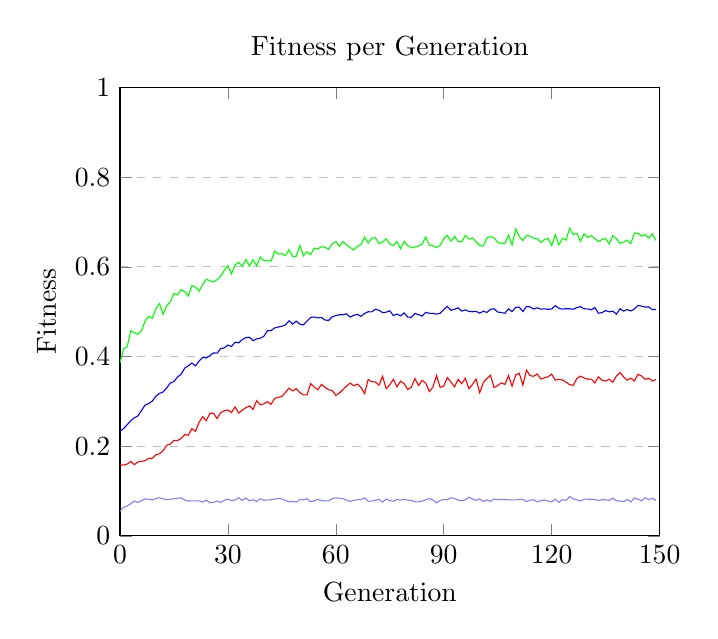
\begin{tikzpicture}
\begin{axis}[
	title={Fitness per Generation},
	xlabel={Generation},
	ylabel={Fitness},
	xmin=0, xmax=150,
	ymin=0, ymax=1,
	xtick={0.0,30.0,60.0,90.0,120.0,150.0},
	ytick={0.0,0.2,0.4,0.6000000000000001,0.8,1.0},
	ymajorgrids=true,
	grid style=dashed,
]

\addplot[
	color=green,
	]
	coordinates {
	(0,0.3854052380952381)(1,0.41743357142857146)(2,0.42157682539682534)(3,0.45713761904761896)(4,0.4532113492063491)(5,0.4495180158730159)(6,0.4580835714285714)(7,0.47940619047619054)(8,0.4897792857142858)(9,0.4855703968253968)(10,0.5073754761904762)(11,0.5182029365079365)(12,0.49415269841269843)(13,0.5134533333333333)(14,0.5221603174603175)(15,0.5406062698412699)(16,0.537418888888889)(17,0.5492764285714286)(18,0.5450616666666667)(19,0.5351248412698414)(20,0.5580815873015872)(21,0.554837619047619)(22,0.5460739682539683)(23,0.5606091269841271)(24,0.5724277777777779)(25,0.5690688095238096)(26,0.5665598412698412)(27,0.5714403174603174)(28,0.5791705555555555)(29,0.5925315873015873)(30,0.6027894444444445)(31,0.584477380952381)(32,0.6045595238095236)(33,0.6099875396825395)(34,0.6015640476190476)(35,0.6165365079365079)(36,0.601628015873016)(37,0.6159319841269841)(38,0.6024546031746031)(39,0.621714365079365)(40,0.614461746031746)(41,0.6140362698412697)(42,0.6129358730158728)(43,0.6350685714285714)(44,0.6287283333333332)(45,0.6293050793650794)(46,0.625271746031746)(47,0.6384260317460317)(48,0.622931507936508)(49,0.6238775396825398)(50,0.6476291269841271)(51,0.624780238095238)(52,0.6335662698412698)(53,0.6272449999999999)(54,0.6416805555555556)(55,0.6399261111111111)(56,0.6450772222222222)(57,0.6434280952380954)(58,0.639648253968254)(59,0.6516123809523808)(60,0.6563689682539684)(61,0.646167380952381)(62,0.6563975396825399)(63,0.6493376190476191)(64,0.6432475396825398)(65,0.6379366666666665)(66,0.6459992857142856)(67,0.6493377777777778)(68,0.6664628571428571)(69,0.6531426190476189)(70,0.6641951587301588)(71,0.6650793650793649)(72,0.6521000000000001)(73,0.6552315079365079)(74,0.6625942857142857)(75,0.6511775396825396)(76,0.6475480952380953)(77,0.6562457142857141)(78,0.6402173015873015)(79,0.656825)(80,0.6475980952380951)(81,0.6428030952380953)(82,0.644273492063492)(83,0.6467825396825397)(84,0.6511092063492065)(85,0.6663246825396826)(86,0.6482075396825396)(87,0.6470598412698413)(88,0.643404126984127)(89,0.648068650793651)(90,0.662906984126984)(91,0.6703600793650794)(92,0.6571707142857144)(93,0.6680363492063492)(94,0.6564643650793651)(95,0.6558188095238094)(96,0.6700690476190476)(97,0.6619723015873015)(98,0.6646146031746032)(99,0.6558840476190476)(100,0.6477884126984126)(101,0.646552380952381)(102,0.6645981746031745)(103,0.6676441269841268)(104,0.6647354761904762)(105,0.654767777777778)(106,0.6520855555555555)(107,0.6523888888888889)(108,0.6708454761904762)(109,0.649092380952381)(110,0.6844784126984128)(111,0.6677857936507936)(112,0.6587338888888888)(113,0.670345873015873)(114,0.6688483333333335)(115,0.6637397619047619)(116,0.663235)(117,0.6547445238095239)(118,0.6607136507936507)(119,0.6636344444444446)(120,0.6479490476190476)(121,0.671520238095238)(122,0.6490583333333333)(123,0.6639530952380952)(124,0.659686111111111)(125,0.6863349206349205)(126,0.6721211904761905)(127,0.6751194444444443)(128,0.6572322222222222)(129,0.6735532539682539)(130,0.6663234126984128)(131,0.6695684126984126)(132,0.6630360317460317)(133,0.6565759523809522)(134,0.6607265873015875)(135,0.6634681746031746)(136,0.6513348412698413)(137,0.6697131746031746)(138,0.6625357936507936)(139,0.6527003174603175)(140,0.655332619047619)(141,0.6596569047619047)(142,0.6520825396825396)(143,0.6752941269841268)(144,0.6749007936507937)(145,0.6685057142857143)(146,0.6720050793650794)(147,0.6644692857142858)(148,0.6735408730158731)(149,0.6590466666666667)
	};
\addplot[
	color=blue,
	]
	coordinates {
	(0,0.23341582010582007)(1,0.23945444444444444)(2,0.24783851851851849)(3,0.25716235119047626)(4,0.26332109788359787)(5,0.2677289186507937)(6,0.27987786375661383)(7,0.2918434656084656)(8,0.2950874107142857)(9,0.30078963955026455)(10,0.3117538624338625)(11,0.3178337202380953)(12,0.32097923941798945)(13,0.3303134788359788)(14,0.3408783333333334)(15,0.3442648544973545)(16,0.35423655423280426)(17,0.36054948743386245)(18,0.3741453207671957)(19,0.37947775793650795)(20,0.3856846428571429)(21,0.37914357473544974)(22,0.39005090277777776)(23,0.39806746362433865)(24,0.39679892857142857)(25,0.40206844246031753)(26,0.4080816236772486)(27,0.40757105489417994)(28,0.41777688822751324)(29,0.41939785714285716)(30,0.4256608399470899)(31,0.42226457671957673)(32,0.4319285251322752)(33,0.43078813161375656)(34,0.43775256613756613)(35,0.4422594113756613)(36,0.4430311342592593)(37,0.43540711309523805)(38,0.43943342592592594)(39,0.44099251653439153)(40,0.4451518882275132)(41,0.45763896825396816)(42,0.45787082671957674)(43,0.463810796957672)(44,0.4658672883597883)(45,0.4676191038359787)(46,0.4706087037037038)(47,0.47974581679894174)(48,0.47251104166666663)(49,0.4789437764550264)(50,0.47230957341269836)(51,0.47077102843915347)(52,0.47925345568783073)(53,0.48728440476190477)(54,0.4883141236772487)(55,0.4861945634920634)(56,0.4871138756613757)(57,0.4814951785714286)(58,0.48069697089947094)(59,0.4886677414021163)(60,0.4913268584656084)(61,0.49314797288359785)(62,0.49346536375661365)(63,0.49527057870370356)(64,0.48800184854497347)(65,0.4921009755291006)(66,0.49410188492063484)(67,0.4896091798941799)(68,0.49599869708994715)(69,0.4999505291005291)(70,0.4996031117724868)(71,0.5054025727513228)(72,0.5034298511904761)(73,0.49797306216931203)(74,0.49894483796296296)(75,0.5021025363756614)(76,0.4913355985449735)(77,0.4946915773809523)(78,0.49103020171957673)(79,0.49725307208994696)(80,0.48806354828042325)(81,0.48760354166666653)(82,0.496124083994709)(83,0.4935297255291005)(84,0.49025646164021164)(85,0.4986593022486772)(86,0.4963995072751324)(87,0.4964763624338623)(88,0.4946208697089947)(89,0.4965806481481483)(90,0.5047905886243387)(91,0.5119165542328042)(92,0.5031410879629629)(93,0.5056456746031748)(94,0.508678664021164)(95,0.5014229894179895)(96,0.5041261772486773)(97,0.5007670436507936)(98,0.49998588955026463)(99,0.5007977777777778)(100,0.4967750198412699)(101,0.501240052910053)(102,0.4984369841269841)(103,0.505365248015873)(104,0.506572833994709)(105,0.49940580687830693)(106,0.49813191798941786)(107,0.4964619146825397)(108,0.5063395403439154)(109,0.5003592328042328)(110,0.5095329133597883)(111,0.51022394510582)(112,0.5003574272486772)(113,0.5117254695767196)(114,0.5107324074074074)(115,0.5060257242063493)(116,0.5087623478835979)(117,0.5057140575396826)(118,0.5064873148148148)(119,0.5053898214285714)(120,0.5059754431216931)(121,0.5137332738095237)(122,0.5075575099206349)(123,0.5057553472222223)(124,0.5067626091269841)(125,0.5066025330687831)(126,0.5055479497354497)(127,0.5092545304232804)(128,0.5113969841269841)(129,0.5065815244708995)(130,0.5063532473544973)(131,0.5042983498677248)(132,0.5092361408730158)(133,0.49663533399470894)(134,0.49816279761904764)(135,0.502575009920635)(136,0.49977334325396816)(137,0.5012650396825398)(138,0.49470442460317465)(139,0.506419484126984)(140,0.5013479166666667)(141,0.5048558366402116)(142,0.501785906084656)(143,0.5060235085978837)(144,0.5141503604497355)(145,0.5124378339947091)(146,0.5103973842592593)(147,0.5105576190476191)(148,0.5047449933862435)(149,0.504938277116402)
	};
\addplot[
	color=red,
	]
	coordinates {
	(0,0.15805380952380957)(1,0.15798388888888887)(2,0.1600922222222222)(3,0.1661516666666667)(4,0.15895992063492068)(5,0.1649728571428571)(6,0.1662018253968254)(7,0.16789111111111116)(8,0.1730022222222222)(9,0.1731411904761904)(10,0.180869365079365)(11,0.1830757142857143)(12,0.19005547619047614)(13,0.20225960317460323)(14,0.2048926984126984)(15,0.21275087301587303)(16,0.21253507936507932)(17,0.21730158730158736)(18,0.22607301587301584)(19,0.22444111111111106)(20,0.23897722222222223)(21,0.23333412698412698)(22,0.2531914285714285)(23,0.2658061904761905)(24,0.25686841269841265)(25,0.27364341269841264)(26,0.2733891269841271)(27,0.2616154761904762)(28,0.2749590476190476)(29,0.27913999999999994)(30,0.2807914285714286)(31,0.27519325396825395)(32,0.28757698412698407)(33,0.2740437301587302)(34,0.28029531746031744)(35,0.2860158730158731)(36,0.2897703174603175)(37,0.28233206349206347)(38,0.30147007936507947)(39,0.2922761904761905)(40,0.29454888888888886)(41,0.29919079365079365)(42,0.2934353174603175)(43,0.3067492857142857)(44,0.3088384126984126)(45,0.3109788888888889)(46,0.32013222222222226)(47,0.32943873015873026)(48,0.32345206349206335)(49,0.32843555555555565)(50,0.31969484126984116)(51,0.3146953968253968)(52,0.3144192063492063)(53,0.3396014285714285)(54,0.3318397619047619)(55,0.3259561111111111)(56,0.33786555555555564)(57,0.331658253968254)(58,0.325785873015873)(59,0.32466817460317454)(60,0.31344333333333335)(61,0.31860079365079363)(62,0.3263800793650794)(63,0.33395619047619046)(64,0.3407312698412698)(65,0.3347949206349207)(66,0.3385203174603174)(67,0.3310021428571429)(68,0.3174053968253968)(69,0.3488382539682539)(70,0.34395785714285715)(71,0.3433549206349207)(72,0.3361536507936508)(73,0.35592753968253965)(74,0.3285948412698413)(75,0.33709968253968253)(76,0.34920444444444443)(77,0.33255388888888887)(78,0.345180634920635)(79,0.33964055555555556)(80,0.3267117460317461)(81,0.3320415873015872)(82,0.3509279365079366)(83,0.3355633333333333)(84,0.3468884126984126)(85,0.3403057142857143)(86,0.32206579365079374)(87,0.3319703968253968)(88,0.3575314285714285)(89,0.33117761904761905)(90,0.3340311111111111)(91,0.3531091269841271)(92,0.34308238095238086)(93,0.3326664285714286)(94,0.3491501587301588)(95,0.339572619047619)(96,0.35145912698412696)(97,0.3284585714285715)(98,0.3381631746031745)(99,0.34999960317460316)(100,0.3194007936507937)(101,0.3419467460317461)(102,0.3511061111111111)(103,0.35817277777777773)(104,0.3308245238095238)(105,0.335285238095238)(106,0.3412398412698412)(107,0.33795277777777766)(108,0.35746373015873023)(109,0.3341884126984127)(110,0.35890785714285717)(111,0.3628196031746031)(112,0.33637103174603167)(113,0.36962071428571425)(114,0.35739984126984137)(115,0.3560751587301589)(116,0.36113031746031743)(117,0.3500217460317461)(118,0.3526938095238096)(119,0.3548763492063492)(120,0.36088174603174605)(121,0.3473142857142857)(122,0.34891865079365086)(123,0.34780952380952385)(124,0.34295690476190477)(125,0.33752103174603176)(126,0.33578674603174613)(127,0.35104507936507934)(128,0.35616952380952377)(129,0.35252301587301593)(130,0.34935190476190475)(131,0.3496787301587301)(132,0.3412313492063492)(133,0.3547953174603174)(134,0.347195873015873)(135,0.34561063492063493)(136,0.3492407142857142)(137,0.34286984126984127)(138,0.3566372222222223)(139,0.3643493650793651)(140,0.35451674603174615)(141,0.3472307936507937)(142,0.35183420634920637)(143,0.34557119047619045)(144,0.36032587301587304)(145,0.35661388888888895)(146,0.34930944444444445)(147,0.35150301587301586)(148,0.3455242063492063)(149,0.3489911904761905)
	};
\addplot[
	color=blue!50,
	]
	coordinates {
	(0,0.054901299845547605)(1,0.06411441249312055)(2,0.06655982056205524)(3,0.07199652265558798)(4,0.07785960977008408)(5,0.07448264641256473)(6,0.07910181082758984)(7,0.08236876444110477)(8,0.08175827540129947)(9,0.08026704656290362)(10,0.0831185299234548)(11,0.08511072867000284)(12,0.08253824178237378)(13,0.08069349543430203)(14,0.08158794474895853)(15,0.08285722979572434)(16,0.08415884788466033)(17,0.08470794426449926)(18,0.08014437372039765)(19,0.07779969071434409)(20,0.07806765013153726)(21,0.07823211490716238)(22,0.07798909624865565)(23,0.07536941280902942)(24,0.0798927974789094)(25,0.07387577854073507)(26,0.07459046010935125)(27,0.07776552146968749)(28,0.07471112099933166)(29,0.0794060734484023)(30,0.08206579060771275)(31,0.07860883069026822)(32,0.07997651316142897)(33,0.08509363382668063)(34,0.07883909262012584)(35,0.08445866751671213)(36,0.07801111482461398)(37,0.08062531923572895)(38,0.07678200341002733)(39,0.08243369007948574)(40,0.07947808498061511)(41,0.08040287843804053)(42,0.08051403797774363)(43,0.08207704515006604)(44,0.08373122552630786)(45,0.08230673127600444)(46,0.07929054592274597)(47,0.07598493411098428)(48,0.0767676027066942)(49,0.0754316771467542)(50,0.08126417832820812)(51,0.0802877365396467)(52,0.08287528317515519)(53,0.07597595231473361)(54,0.07828561343893967)(55,0.08128943354289052)(56,0.07891823630850497)(57,0.0781378786552582)(58,0.07819997712559311)(59,0.0832372862600825)(60,0.08480495762503225)(61,0.08412315043243616)(62,0.08275863768476331)(63,0.08011512743399074)(64,0.07672043392543922)(65,0.07949971532020567)(66,0.08059741265679057)(67,0.0810988950378033)(68,0.08473379607261049)(69,0.07734776020400012)(70,0.07761647464907029)(71,0.07940917382752717)(72,0.08147429787022571)(73,0.07499777186328274)(74,0.08245526035034005)(75,0.07866269358576122)(76,0.07724554044985779)(77,0.08130452827373005)(78,0.07965027484469396)(79,0.08174042721877514)(80,0.07973370191107185)(81,0.07931816658441587)(82,0.07581976391220452)(83,0.07598149724379231)(84,0.07745070549187023)(85,0.08055296329685892)(86,0.08301905532779191)(87,0.08042208071164476)(88,0.07364336573176647)(89,0.07904528804428837)(90,0.08115463500532287)(91,0.08036678000639456)(92,0.08521510854287626)(93,0.08313050739357976)(94,0.07968652513752095)(95,0.07881087292583264)(96,0.08031305482629213)(97,0.08608792563659728)(98,0.08216663099061844)(99,0.07935819957297928)(100,0.08249752183415829)(101,0.07684604623791752)(102,0.08014567273685397)(103,0.07728960611293927)(104,0.0820591455461682)(105,0.08097046920979523)(106,0.08161484464809739)(107,0.08107212105821088)(108,0.08038419511118307)(109,0.08024534762082762)(110,0.0802296561095919)(111,0.08131895116959786)(112,0.08142293603587103)(113,0.07669717192544961)(114,0.07970129742358989)(115,0.08048550581089028)(116,0.07584218701935354)(117,0.07876050190014527)(118,0.08015475690175417)(119,0.07775114064561323)(120,0.0756766742276645)(121,0.08177976514340028)(122,0.07483010082813475)(123,0.08105791712535086)(124,0.07924585758478042)(125,0.08779714954179542)(126,0.08268689561129135)(127,0.08074621022209912)(128,0.07781683823667666)(129,0.08183925493647207)(130,0.08188356559396069)(131,0.081469382717169)(132,0.08105927808404978)(133,0.0790191543877171)(134,0.0806126206984968)(135,0.08046559869872327)(136,0.0792349257157087)(137,0.0843099756511807)(138,0.07829753798354902)(139,0.0776950892313251)(140,0.07662964252015908)(141,0.08119862365834848)(142,0.0756914918749451)(143,0.08475610167240939)(144,0.08183239889228806)(145,0.07835718056821717)(146,0.08485622720402053)(147,0.08084384975864646)(148,0.08415944598028657)(149,0.0789308387006915)
	};
\end{axis}
\end{tikzpicture}
}
		\caption{Some sample caption}
	\end{subfigure}%
}
\end{figure}

\newpage
\vspace*{-2.0cm}
\textbf{\Huge LARGE SAMPLE HEADER}
\vspace{1.5cm}
\begin{tikzpicture}[remember picture,overlay]
   \node[anchor=south east,inner sep=20pt] at (current page.south east)
              {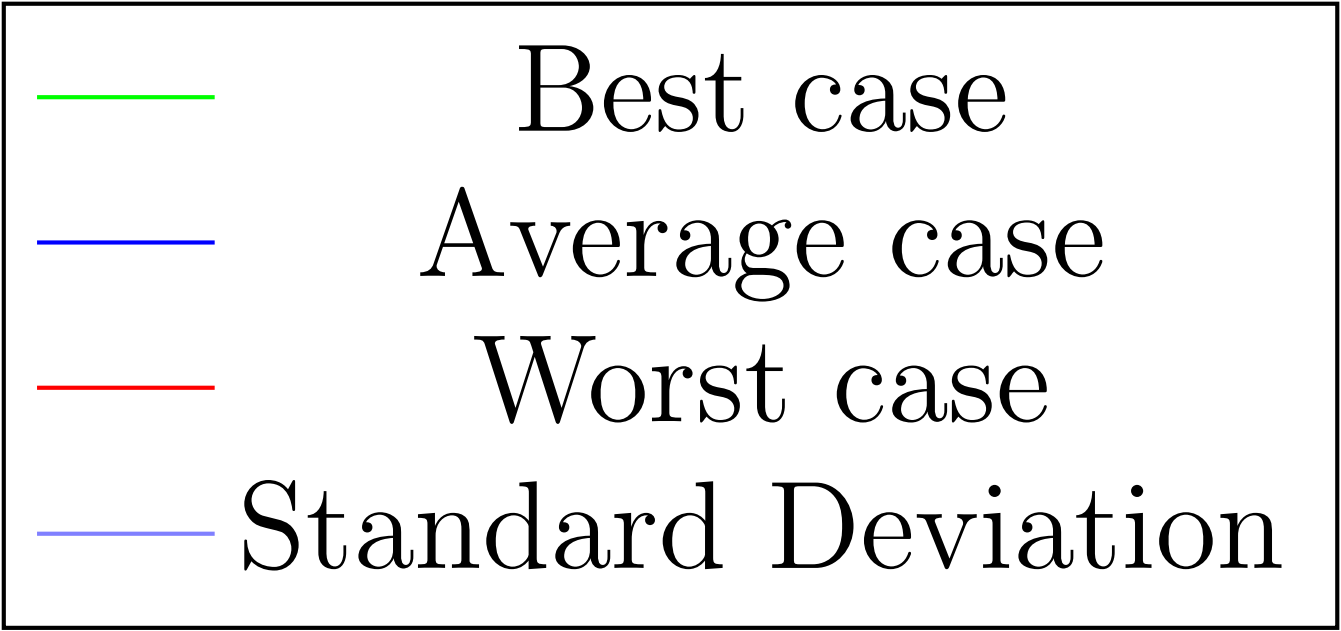
\includegraphics[scale=0.1]{chapters/res/generated_graph_legend.png}};
\end{tikzpicture}

\begin{figure}[H]
\vspace*{-1cm}
	\makebox[\linewidth][c]{%
	\begin{subfigure}[b]{0.7\textwidth}
		\centering
		\resizebox{0.9\linewidth}{!}{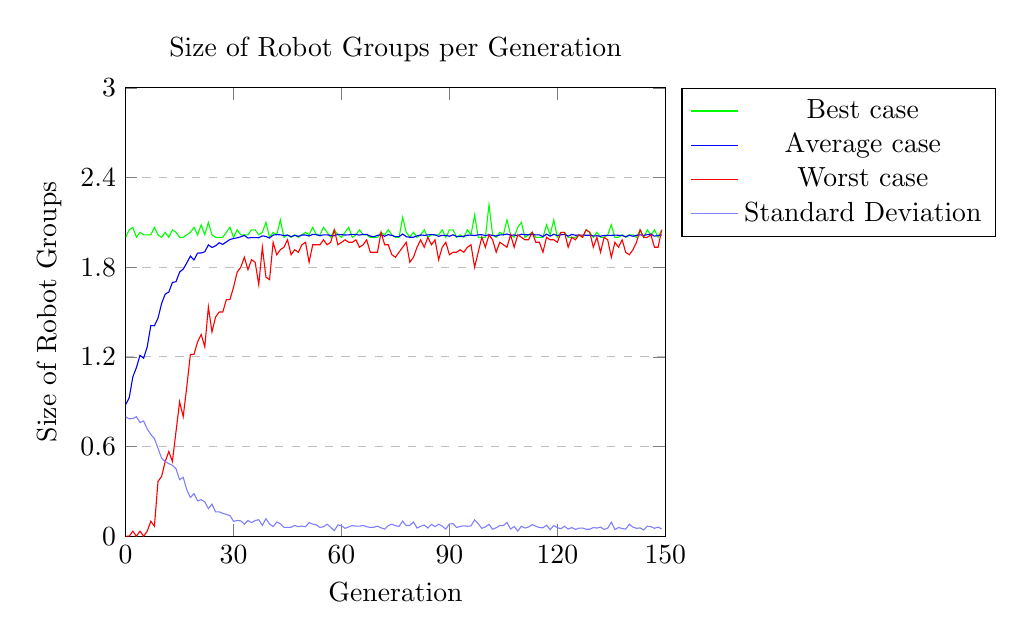
\begin{tikzpicture}
\begin{axis}[
	title={Size of Robot Groups per Generation},
	xlabel={Generation},
	ylabel={Size of Robot Groups},
	xmin=0, xmax=150,
	ymin=0, ymax=3,
	xtick={0.0,30.0,60.0,90.0,120.0,150.0},
	ytick={0.0,0.6,1.2,1.7999999999999998,2.4,3.0},
	legend pos=outer north east,
	ymajorgrids=true,
	grid style=dashed,
]

\addplot[
	color=green,
	]
	coordinates {
	(0,2.0000000000000004)(1,2.0500000000000003)(2,2.0666666666666673)(3,2.0000000000000004)(4,2.033333333333334)(5,2.016666666666667)(6,2.016666666666667)(7,2.0166666666666675)(8,2.0666666666666673)(9,2.016666666666667)(10,2.0000000000000004)(11,2.033333333333334)(12,2.0000000000000004)(13,2.0500000000000007)(14,2.0333333333333337)(15,2.0000000000000004)(16,2.0000000000000004)(17,2.0166666666666675)(18,2.033333333333334)(19,2.0666666666666673)(20,2.016666666666667)(21,2.083333333333334)(22,2.016666666666667)(23,2.1)(24,2.0166666666666675)(25,2.0000000000000004)(26,2.0000000000000004)(27,2.0000000000000004)(28,2.033333333333334)(29,2.0666666666666673)(30,2.0000000000000004)(31,2.0500000000000007)(32,2.016666666666667)(33,2.0166666666666675)(34,2.016666666666667)(35,2.0500000000000007)(36,2.0500000000000003)(37,2.016666666666667)(38,2.033333333333334)(39,2.100000000000001)(40,2.0000000000000004)(41,2.0333333333333337)(42,2.016666666666667)(43,2.116666666666667)(44,2.0000000000000004)(45,2.0166666666666675)(46,2.0000000000000004)(47,2.016666666666667)(48,2.0000000000000004)(49,2.0166666666666675)(50,2.033333333333334)(51,2.016666666666667)(52,2.0666666666666673)(53,2.016666666666667)(54,2.0166666666666675)(55,2.0666666666666673)(56,2.033333333333334)(57,2.0000000000000004)(58,2.0500000000000007)(59,2.016666666666667)(60,2.0000000000000004)(61,2.033333333333334)(62,2.0666666666666673)(63,2.0000000000000004)(64,2.0166666666666675)(65,2.0500000000000003)(66,2.0166666666666675)(67,2.016666666666667)(68,2.0000000000000004)(69,2.0000000000000004)(70,2.0000000000000004)(71,2.033333333333334)(72,2.016666666666667)(73,2.0500000000000007)(74,2.0166666666666675)(75,2.0000000000000004)(76,2.0000000000000004)(77,2.1333333333333337)(78,2.033333333333334)(79,2.0000000000000004)(80,2.033333333333334)(81,2.0000000000000004)(82,2.0166666666666675)(83,2.0500000000000003)(84,2.0000000000000004)(85,2.0166666666666675)(86,2.016666666666667)(87,2.016666666666667)(88,2.0500000000000007)(89,2.0000000000000004)(90,2.0500000000000007)(91,2.0500000000000007)(92,2.0000000000000004)(93,2.016666666666667)(94,2.0000000000000004)(95,2.0500000000000003)(96,2.016666666666667)(97,2.150000000000001)(98,2.0000000000000004)(99,2.0000000000000004)(100,2.0000000000000004)(101,2.216666666666667)(102,2.0166666666666675)(103,2.0000000000000004)(104,2.033333333333334)(105,2.0166666666666675)(106,2.1166666666666676)(107,2.0166666666666675)(108,2.0000000000000004)(109,2.0666666666666673)(110,2.1)(111,2.0000000000000004)(112,2.0166666666666675)(113,2.033333333333334)(114,2.0000000000000004)(115,2.0000000000000004)(116,2.0000000000000004)(117,2.0833333333333344)(118,2.0166666666666675)(119,2.1166666666666676)(120,2.0000000000000004)(121,2.033333333333334)(122,2.033333333333334)(123,2.0000000000000004)(124,2.0000000000000004)(125,2.0000000000000004)(126,2.016666666666667)(127,2.0000000000000004)(128,2.0500000000000007)(129,2.033333333333334)(130,2.0000000000000004)(131,2.033333333333334)(132,2.0000000000000004)(133,2.0000000000000004)(134,2.0166666666666675)(135,2.083333333333334)(136,2.0000000000000004)(137,2.0000000000000004)(138,2.016666666666667)(139,2.0000000000000004)(140,2.0166666666666675)(141,2.016666666666667)(142,2.0000000000000004)(143,2.0500000000000007)(144,2.0000000000000004)(145,2.0500000000000007)(146,2.016666666666667)(147,2.0500000000000003)(148,2.0000000000000004)(149,2.0500000000000007)
	};
	\addlegendentry{Best case}
\addplot[
	color=blue,
	]
	coordinates {
	(0,0.8798611111111109)(1,0.9270833333333335)(2,1.065972222222222)(3,1.1284722222222223)(4,1.2104166666666665)(5,1.190972222222222)(6,1.2666666666666666)(7,1.4097222222222223)(8,1.4083333333333334)(9,1.4590277777777778)(10,1.5576388888888886)(11,1.6201388888888886)(12,1.6333333333333335)(13,1.697916666666667)(14,1.7027777777777782)(15,1.7673611111111112)(16,1.7868055555555558)(17,1.8291666666666666)(18,1.8743055555555561)(19,1.8486111111111116)(20,1.8944444444444448)(21,1.8951388888888892)(22,1.9034722222222227)(23,1.9493055555555558)(24,1.9319444444444447)(25,1.943055555555556)(26,1.9631944444444447)(27,1.9527777777777782)(28,1.9694444444444448)(29,1.9854166666666675)(30,1.991666666666667)(31,1.9965277777777781)(32,2.0034722222222223)(33,2.013194444444445)(34,1.995138888888889)(35,1.9986111111111116)(36,1.9979166666666666)(37,1.9972222222222227)(38,2.0097222222222224)(39,2.005555555555556)(40,1.9951388888888892)(41,2.015277777777778)(42,2.0180555555555557)(43,2.016666666666667)(44,2.0125000000000006)(45,2.0145833333333334)(46,2.0041666666666673)(47,2.0131944444444447)(48,2.0062500000000005)(49,2.0152777777777784)(50,2.0152777777777784)(51,2.009027777777778)(52,2.019444444444445)(53,2.018055555555556)(54,2.010416666666667)(55,2.016666666666667)(56,2.016666666666667)(57,2.0118055555555556)(58,2.010416666666667)(59,2.0201388888888894)(60,2.0173611111111116)(61,2.0152777777777784)(62,2.016666666666667)(63,2.019444444444445)(64,2.0187500000000003)(65,2.014583333333334)(66,2.0201388888888894)(67,2.019444444444445)(68,2.0083333333333337)(69,2.0034722222222228)(70,2.0131944444444447)(71,2.017361111111111)(72,2.0069444444444446)(73,2.018055555555556)(74,2.0125000000000006)(75,2.0048611111111114)(76,2.0048611111111114)(77,2.0222222222222226)(78,2.0041666666666673)(79,2.0000000000000004)(80,2.0006944444444446)(81,2.0097222222222224)(82,2.0159722222222225)(83,2.013194444444445)(84,2.0159722222222225)(85,2.0187500000000003)(86,2.0159722222222225)(87,2.0069444444444446)(88,2.0131944444444447)(89,2.0131944444444447)(90,2.0069444444444446)(91,2.016666666666667)(92,2.005555555555556)(93,2.005555555555556)(94,2.0069444444444446)(95,2.0138888888888893)(96,2.0145833333333334)(97,2.0118055555555556)(98,2.016666666666667)(99,2.0173611111111116)(100,2.0111111111111115)(101,2.017361111111111)(102,2.0125000000000006)(103,2.0083333333333337)(104,2.0159722222222225)(105,2.016666666666667)(106,2.0222222222222226)(107,2.013194444444445)(108,2.0159722222222225)(109,2.0111111111111115)(110,2.020833333333334)(111,2.0173611111111116)(112,2.016666666666667)(113,2.0208333333333335)(114,2.015972222222223)(115,2.0159722222222225)(116,2.0048611111111114)(117,2.020833333333334)(118,2.007638888888889)(119,2.0201388888888894)(120,2.0118055555555556)(121,2.016666666666667)(122,2.020138888888889)(123,2.007638888888889)(124,2.0194444444444453)(125,2.0138888888888893)(126,2.014583333333334)(127,2.0145833333333334)(128,2.0138888888888893)(129,2.013888888888889)(130,2.009027777777778)(131,2.010416666666667)(132,2.006944444444445)(133,2.0131944444444447)(134,2.0125000000000006)(135,2.0131944444444447)(136,2.014583333333334)(137,2.0138888888888893)(138,2.0118055555555556)(139,2.0041666666666673)(140,2.013888888888889)(141,2.006944444444445)(142,2.013194444444445)(143,2.016666666666667)(144,2.0125000000000006)(145,2.0180555555555557)(146,2.021527777777778)(147,2.007638888888889)(148,2.0125)(149,2.0159722222222225)
	};
	\addlegendentry{Average case}
\addplot[
	color=red,
	]
	coordinates {
	(0,0.0)(1,0.0)(2,0.03333333333333333)(3,0.0)(4,0.03333333333333333)(5,0.0)(6,0.03333333333333333)(7,0.1)(8,0.06666666666666667)(9,0.3666666666666667)(10,0.4)(11,0.49999999999999994)(12,0.5666666666666667)(13,0.5)(14,0.7)(15,0.8999999999999999)(16,0.7999999999999999)(17,0.9999999999999999)(18,1.2166666666666668)(19,1.2166666666666668)(20,1.3)(21,1.35)(22,1.2666666666666666)(23,1.5333333333333334)(24,1.3666666666666667)(25,1.4666666666666668)(26,1.5000000000000002)(27,1.5000000000000002)(28,1.5833333333333337)(29,1.5833333333333335)(30,1.666666666666667)(31,1.766666666666667)(32,1.8000000000000005)(33,1.8666666666666671)(34,1.7833333333333339)(35,1.8500000000000008)(36,1.833333333333334)(37,1.6833333333333336)(38,1.9333333333333338)(39,1.7333333333333338)(40,1.716666666666667)(41,1.9666666666666672)(42,1.8833333333333337)(43,1.9166666666666672)(44,1.933333333333334)(45,1.983333333333334)(46,1.883333333333334)(47,1.9166666666666672)(48,1.9000000000000006)(49,1.9500000000000006)(50,1.9666666666666672)(51,1.833333333333334)(52,1.9500000000000006)(53,1.9500000000000006)(54,1.9500000000000006)(55,1.983333333333334)(56,1.9500000000000006)(57,1.9666666666666675)(58,2.0500000000000007)(59,1.9500000000000006)(60,1.9666666666666675)(61,1.983333333333334)(62,1.9666666666666675)(63,1.9666666666666672)(64,1.983333333333334)(65,1.933333333333334)(66,1.9500000000000006)(67,1.983333333333334)(68,1.9000000000000006)(69,1.9000000000000006)(70,1.9000000000000004)(71,2.033333333333334)(72,1.9500000000000004)(73,1.9500000000000006)(74,1.883333333333334)(75,1.8666666666666671)(76,1.9000000000000008)(77,1.9333333333333342)(78,1.9666666666666675)(79,1.833333333333334)(80,1.8666666666666674)(81,1.933333333333334)(82,1.983333333333334)(83,1.9333333333333338)(84,2.0000000000000004)(85,1.9500000000000008)(86,1.983333333333334)(87,1.8500000000000003)(88,1.9333333333333338)(89,1.9666666666666672)(90,1.883333333333334)(91,1.9000000000000006)(92,1.9000000000000006)(93,1.9166666666666672)(94,1.9000000000000004)(95,1.933333333333334)(96,1.9500000000000004)(97,1.8000000000000005)(98,1.9000000000000006)(99,2.0000000000000004)(100,1.933333333333334)(101,2.016666666666667)(102,1.983333333333334)(103,1.9000000000000006)(104,1.9666666666666672)(105,1.9500000000000006)(106,1.933333333333334)(107,2.0166666666666675)(108,1.933333333333334)(109,2.016666666666667)(110,2.0000000000000004)(111,1.9833333333333338)(112,1.983333333333334)(113,2.033333333333334)(114,1.9666666666666675)(115,1.9666666666666672)(116,1.9000000000000008)(117,2.000000000000001)(118,1.983333333333334)(119,1.983333333333334)(120,1.9666666666666672)(121,2.033333333333334)(122,2.033333333333334)(123,1.933333333333334)(124,2.0000000000000004)(125,1.983333333333334)(126,2.016666666666667)(127,2.0000000000000004)(128,2.0500000000000007)(129,2.033333333333334)(130,1.933333333333334)(131,2.0000000000000004)(132,1.9000000000000006)(133,2.0000000000000004)(134,1.983333333333334)(135,1.8666666666666671)(136,1.9666666666666672)(137,1.933333333333334)(138,1.983333333333334)(139,1.9000000000000006)(140,1.883333333333334)(141,1.9166666666666672)(142,1.9666666666666672)(143,2.0500000000000007)(144,2.0000000000000004)(145,2.0000000000000004)(146,2.016666666666667)(147,1.933333333333334)(148,1.9333333333333338)(149,2.0500000000000007)
	};
	\addlegendentry{Worst case}
\addplot[
	color=blue!50,
	]
	coordinates {
	(0,0.7983311755495729)(1,0.7855423863953697)(2,0.7871253815576873)(3,0.7993947144540696)(4,0.7607876356614588)(5,0.771121278903698)(6,0.7173637423564808)(7,0.6805657166864519)(8,0.6536032240985181)(9,0.5881336499750809)(10,0.522056049245939)(11,0.498929027559466)(12,0.4858452636748676)(13,0.47426272476363873)(14,0.4513992046882054)(15,0.3783832537381997)(16,0.39384225446691024)(17,0.31048799645347164)(18,0.2590721203711587)(19,0.28441688256920156)(20,0.2363118528974239)(21,0.24450045613956498)(22,0.22899622710176998)(23,0.18444716314296203)(24,0.21439099799215794)(25,0.16250380986475277)(26,0.16288251381517108)(27,0.1525886568336205)(28,0.1461005948903228)(29,0.13774057959377478)(30,0.09935192773515408)(31,0.10506597780370139)(32,0.10271112307798994)(33,0.08070167915624644)(34,0.1049299510813909)(35,0.09080447963431791)(36,0.10483896386180852)(37,0.11018124736037944)(38,0.07233578380873369)(39,0.1172302362616263)(40,0.08175385336604217)(41,0.06407846802894583)(42,0.09452894622226322)(43,0.08388685928532247)(44,0.05895403092354805)(45,0.05861265956460498)(46,0.05994685633484004)(47,0.07195681098401753)(48,0.06393733203827232)(49,0.06737496015590203)(50,0.06359759902837278)(51,0.09101916664136402)(52,0.08115267548306442)(53,0.07609174654563443)(54,0.058076558300094255)(55,0.0635479747400224)(56,0.08023636355558941)(57,0.059296514552138094)(58,0.03697210013558607)(59,0.07549963892319081)(60,0.06970398860378861)(61,0.0525757399972869)(62,0.062197966765405406)(63,0.07081355584902373)(64,0.06746860557348561)(65,0.06697142609279465)(66,0.07231793396942153)(67,0.06327185523854088)(68,0.05818149233540158)(69,0.0602275734107459)(70,0.06669822649965446)(71,0.056140135218514034)(72,0.04695352688510336)(73,0.07126311549110305)(74,0.07998629605061357)(75,0.07080336741015113)(76,0.06519777057108839)(77,0.10077294522411565)(78,0.070921009470098)(79,0.07273177330726799)(80,0.09534162990198641)(81,0.05433621068542154)(82,0.06677302050007788)(83,0.07455005537166758)(84,0.054564230976556626)(85,0.07920427313409775)(86,0.06376971228479242)(87,0.07984576369931783)(88,0.0667604519691524)(89,0.04775001047577603)(90,0.08185074402210286)(91,0.08377458885323448)(92,0.058239451988007646)(93,0.06481755528041662)(94,0.06942397860035467)(95,0.06654046261217178)(96,0.06883183128967238)(97,0.10901646668949469)(98,0.083468000038766)(99,0.05260108809622554)(100,0.06239267530067373)(101,0.07940802265262764)(102,0.046699935379844626)(103,0.05635761222544963)(104,0.07081058878460422)(105,0.07122368479476444)(106,0.09199269193524985)(107,0.04790629418434261)(108,0.06511086041378902)(109,0.03393267338885214)(110,0.06678030073406985)(111,0.05430261734104916)(112,0.06188929379003112)(113,0.07706023784286557)(114,0.06685709526773043)(115,0.057518442950805874)(116,0.05613733780994192)(117,0.07363665914908524)(118,0.043793216980518676)(119,0.0710549004894864)(120,0.05687163457239522)(121,0.05048831357126835)(122,0.06627967438396375)(123,0.048095556230850454)(124,0.057559415354062865)(125,0.04548610419268803)(126,0.05358149285733128)(127,0.0545671713000547)(128,0.04642112856009753)(129,0.04663698225927933)(130,0.05764983499075631)(131,0.05438977845065981)(132,0.061140232585419174)(133,0.045116171422411554)(134,0.05391038471281062)(135,0.09401177183242798)(136,0.044812624133544074)(137,0.05805463242722705)(138,0.051609393535579466)(139,0.04732865859134238)(140,0.07987567175003345)(141,0.0608128956302697)(142,0.052761489495149756)(143,0.05527316217652164)(144,0.04194473510807866)(145,0.0666473349355931)(146,0.06382806510689948)(147,0.052632647136887735)(148,0.061008484719322104)(149,0.04807421234316709)
	};
	\addlegendentry{Standard Deviation}
\end{axis}
\end{tikzpicture}
}
		\caption{Some sample caption}
	\end{subfigure}%
	\begin{subfigure}[b]{0.7\textwidth}
		\centering
		\resizebox{0.9\linewidth}{!}{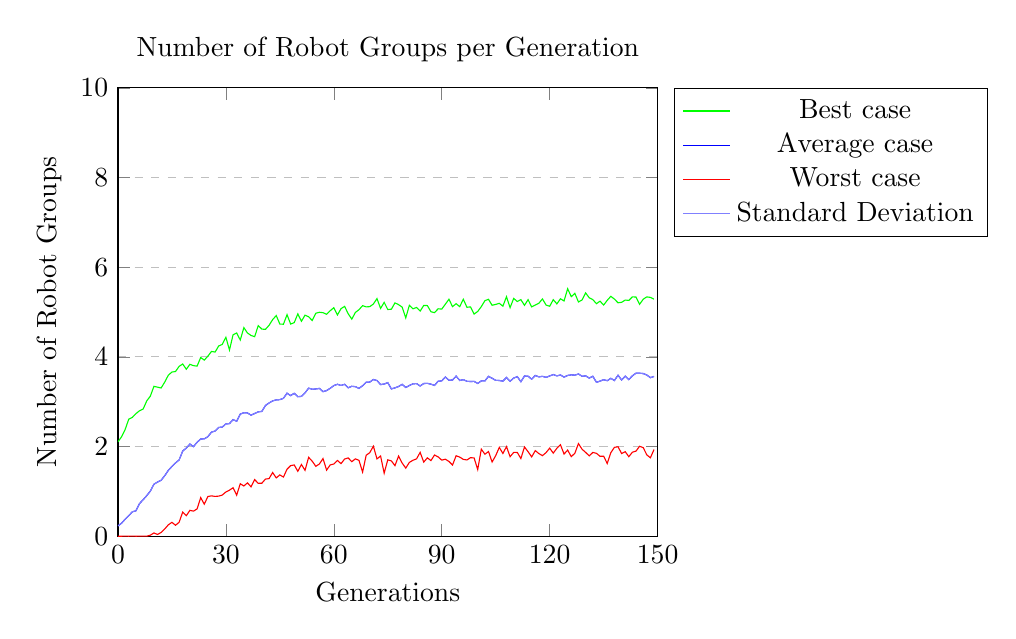
\begin{tikzpicture}
\begin{axis}[
	title={Number of Robot Groups per Generation},
	xlabel={Generations},
	ylabel={Number of Robot Groups},
	xmin=0, xmax=150,
	ymin=0, ymax=10,
	xtick={0.0,30.0,60.0,90.0,120.0,150.0},
	ytick={0.0,2.0,4.0,6.0,8.0,10.0},
	legend pos=outer north east,
	ymajorgrids=true,
	grid style=dashed,
]

\addplot[
	color=green,
	]
	coordinates {
	(0,2.103833333333333)(1,2.216666666666667)(2,2.3800833333333333)(3,2.6098333333333326)(4,2.6499166666666665)(5,2.7333333333333343)(6,2.7982499999999995)(7,2.8364166666666666)(8,3.017083333333333)(9,3.1240000000000006)(10,3.342416666666667)(11,3.324916666666666)(12,3.305166666666667)(13,3.4375833333333334)(14,3.5911666666666675)(15,3.66125)(16,3.6731666666666665)(17,3.7879166666666673)(18,3.8410833333333327)(19,3.723999999999999)(20,3.833333333333333)(21,3.8041666666666663)(22,3.793333333333334)(23,3.9860833333333336)(24,3.927666666666667)(25,4.016333333333334)(26,4.121333333333333)(27,4.106750000000001)(28,4.242916666666666)(29,4.2780000000000005)(30,4.437916666666666)(31,4.15275)(32,4.493583333333333)(33,4.5334166666666675)(34,4.375583333333333)(35,4.652416666666667)(36,4.533)(37,4.476916666666666)(38,4.4505)(39,4.698250000000001)(40,4.618916666666667)(41,4.6137500000000005)(42,4.703416666666666)(43,4.830666666666667)(44,4.92175)(45,4.73125)(46,4.727916666666668)(47,4.941166666666667)(48,4.732)(49,4.764083333333333)(50,4.9588333333333345)(51,4.793916666666665)(52,4.93)(53,4.894833333333334)(54,4.8105)(55,4.973083333333333)(56,4.9946666666666655)(57,4.985666666666667)(58,4.949416666666667)(59,5.0295)(60,5.096916666666667)(61,4.933249999999999)(62,5.074750000000002)(63,5.126500000000001)(64,4.9615833333333335)(65,4.842083333333333)(66,4.990583333333333)(67,5.052583333333333)(68,5.1418333333333335)(69,5.1152500000000005)(70,5.119999999999999)(71,5.179666666666667)(72,5.299416666666666)(73,5.080666666666666)(74,5.21575)(75,5.055833333333333)(76,5.063583333333333)(77,5.204416666666668)(78,5.165333333333334)(79,5.1098333333333334)(80,4.868416666666666)(81,5.149500000000001)(82,5.071250000000001)(83,5.102166666666666)(84,5.021166666666668)(85,5.146583333333332)(86,5.144500000000001)(87,5.006916666666667)(88,4.986083333333333)(89,5.07275)(90,5.064916666666666)(91,5.174499999999999)(92,5.285)(93,5.12075)(94,5.186333333333333)(95,5.120583333333334)(96,5.285416666666667)(97,5.106416666666667)(98,5.115500000000001)(99,4.954916666666665)(100,5.01225)(101,5.121000000000001)(102,5.2535)(103,5.284333333333334)(104,5.150916666666667)(105,5.169999999999999)(106,5.194166666666666)(107,5.131416666666667)(108,5.341666666666668)(109,5.098000000000001)(110,5.303833333333333)(111,5.235166666666667)(112,5.276083333333332)(113,5.150333333333332)(114,5.2763333333333335)(115,5.1146666666666665)(116,5.1570833333333335)(117,5.195749999999999)(118,5.292583333333334)(119,5.155916666666666)(120,5.127916666666668)(121,5.27575)(122,5.181750000000001)(123,5.2950833333333325)(124,5.2475000000000005)(125,5.520000000000001)(126,5.3421666666666665)(127,5.417333333333334)(128,5.22425)(129,5.269416666666666)(130,5.426500000000001)(131,5.317749999999999)(132,5.276916666666668)(133,5.186666666666666)(134,5.2420833333333325)(135,5.1555833333333325)(136,5.26075)(137,5.351083333333333)(138,5.287999999999999)(139,5.206999999999999)(140,5.2165)(141,5.267250000000001)(142,5.258666666666667)(143,5.3382499999999995)(144,5.334666666666666)(145,5.1725)(146,5.285583333333334)(147,5.337916666666667)(148,5.3265)(149,5.287083333333333)
	};
	\addlegendentry{Best case}
\addplot[
	color=blue,
	]
	coordinates {
	(0,0.22944444444444445)(1,0.2897256944444444)(2,0.3776875)(3,0.45748263888888885)(4,0.5443437499999999)(5,0.5652222222222223)(6,0.7281284722222222)(7,0.8133958333333332)(8,0.9048298611111111)(9,1.0064652777777778)(10,1.1595208333333333)(11,1.20740625)(12,1.2472430555555558)(13,1.3494340277777779)(14,1.4696145833333332)(15,1.5540312499999998)(16,1.6347048611111112)(17,1.7002013888888887)(18,1.9000243055555552)(19,1.9661909722222215)(20,2.055034722222222)(21,1.9968229166666667)(22,2.0951319444444447)(23,2.1680451388888886)(24,2.1707083333333337)(25,2.220381944444444)(26,2.3215555555555563)(27,2.34546875)(28,2.42478125)(29,2.4347499999999997)(30,2.504520833333333)(31,2.511840277777778)(32,2.600440972222223)(33,2.5641805555555552)(34,2.7248159722222227)(35,2.753475694444445)(36,2.749263888888889)(37,2.699975694444445)(38,2.7366666666666664)(39,2.7738472222222224)(40,2.7836388888888886)(41,2.914875)(42,2.971628472222222)(43,3.0177013888888884)(44,3.040899305555555)(45,3.0462638888888893)(46,3.0754062499999995)(47,3.1897847222222224)(48,3.135729166666667)(49,3.1878090277777784)(50,3.111611111111111)(51,3.1188611111111113)(52,3.195375)(53,3.3019270833333327)(54,3.2778888888888877)(55,3.2840381944444443)(56,3.2968854166666666)(57,3.2238750000000005)(58,3.2483749999999993)(59,3.2988854166666663)(60,3.359409722222222)(61,3.3888368055555556)(62,3.3633055555555544)(63,3.3872986111111114)(64,3.310559027777778)(65,3.343572916666667)(66,3.3356597222222226)(67,3.2969131944444445)(68,3.3565069444444444)(69,3.4367465277777773)(70,3.4385138888888886)(71,3.4944444444444454)(72,3.4721215277777775)(73,3.381340277777778)(74,3.3942430555555547)(75,3.4257395833333337)(76,3.285527777777778)(77,3.3085208333333336)(78,3.3395347222222225)(79,3.386673611111111)(80,3.317909722222223)(81,3.360357638888889)(82,3.399354166666667)(83,3.403611111111111)(84,3.351138888888888)(85,3.4049895833333332)(86,3.410024305555556)(87,3.3914375000000003)(88,3.363243055555556)(89,3.456694444444444)(90,3.464361111111111)(91,3.5504583333333333)(92,3.479260416666666)(93,3.4847847222222224)(94,3.570934027777777)(95,3.473482638888888)(96,3.49190625)(97,3.455409722222222)(98,3.4501562499999996)(99,3.4527673611111114)(100,3.407545138888889)(101,3.4642152777777775)(102,3.4629930555555557)(103,3.5658090277777776)(104,3.5228090277777775)(105,3.4762881944444444)(106,3.473281250000001)(107,3.458930555555556)(108,3.5397361111111114)(109,3.456211805555555)(110,3.526486111111111)(111,3.5589861111111114)(112,3.4459375000000003)(113,3.5729270833333326)(114,3.569180555555555)(115,3.501447916666667)(116,3.5862013888888895)(117,3.5537916666666667)(118,3.565930555555556)(119,3.5427569444444442)(120,3.573777777777778)(121,3.605694444444445)(122,3.575979166666667)(123,3.595725694444444)(124,3.5488923611111107)(125,3.585704861111111)(126,3.5982222222222227)(127,3.5927708333333337)(128,3.6184236111111123)(129,3.5678958333333335)(130,3.5761909722222223)(131,3.5271249999999994)(132,3.5677812500000003)(133,3.4326111111111115)(134,3.4602361111111106)(135,3.4899444444444447)(136,3.4688472222222217)(137,3.5216875)(138,3.4723472222222225)(139,3.590329861111111)(140,3.483791666666667)(141,3.5689027777777773)(142,3.4936805555555557)(143,3.5777569444444453)(144,3.635972222222222)(145,3.634888888888889)(146,3.628263888888889)(147,3.595222222222222)(148,3.5355312500000005)(149,3.5628298611111107)
	};
	\addlegendentry{Average case}
\addplot[
	color=red,
	]
	coordinates {
	(0,0.0)(1,0.0)(2,8.333333333333334e-05)(3,0.0)(4,0.00025)(5,0.0)(6,8.333333333333334e-05)(7,0.0005833333333333334)(8,0.0004166666666666667)(9,0.021999999999999995)(10,0.07250000000000001)(11,0.03866666666666666)(12,0.08299999999999999)(13,0.16100000000000003)(14,0.2535833333333333)(15,0.3096666666666666)(16,0.24358333333333332)(17,0.31016666666666665)(18,0.5371666666666667)(19,0.4579166666666667)(20,0.5768333333333332)(21,0.5585833333333333)(22,0.6091666666666667)(23,0.8601666666666667)(24,0.7145833333333332)(25,0.8856666666666666)(26,0.8995000000000001)(27,0.8875)(28,0.8935000000000001)(29,0.9179166666666667)(30,0.9866666666666666)(31,1.0267500000000003)(32,1.0817499999999998)(33,0.9157500000000001)(34,1.1696666666666666)(35,1.1197500000000002)(36,1.1895)(37,1.1004166666666668)(38,1.2616666666666667)(39,1.17925)(40,1.1820833333333332)(41,1.2743333333333335)(42,1.284333333333333)(43,1.4205833333333335)(44,1.301)(45,1.3671666666666669)(46,1.3190833333333336)(47,1.4948333333333337)(48,1.5737499999999998)(49,1.5891666666666664)(50,1.44725)(51,1.5998333333333334)(52,1.4684166666666667)(53,1.7594166666666666)(54,1.6724166666666664)(55,1.558583333333333)(56,1.6108333333333333)(57,1.7317500000000001)(58,1.4739999999999998)(59,1.59)(60,1.6098333333333332)(61,1.6898333333333329)(62,1.618583333333333)(63,1.721083333333333)(64,1.7460833333333332)(65,1.66175)(66,1.7253333333333332)(67,1.6913333333333334)(68,1.431)(69,1.8051666666666668)(70,1.8641666666666665)(71,2.0075833333333333)(72,1.7241666666666666)(73,1.7897500000000002)(74,1.4050000000000002)(75,1.7044166666666667)(76,1.679)(77,1.5738333333333336)(78,1.7866666666666664)(79,1.6311666666666667)(80,1.5184999999999995)(81,1.6459166666666667)(82,1.6938333333333335)(83,1.7250833333333333)(84,1.8694166666666667)(85,1.6520833333333331)(86,1.7480000000000002)(87,1.6864999999999999)(88,1.811416666666667)(89,1.7689166666666667)(90,1.6967500000000002)(91,1.7171666666666667)(92,1.6676666666666669)(93,1.587916666666667)(94,1.794583333333333)(95,1.7643333333333333)(96,1.7137500000000003)(97,1.7004166666666662)(98,1.7519166666666672)(99,1.7451666666666668)(100,1.48625)(101,1.94125)(102,1.8288333333333333)(103,1.8883333333333336)(104,1.6548333333333334)(105,1.7970833333333334)(106,1.9809166666666667)(107,1.8455000000000001)(108,1.9979166666666666)(109,1.7736666666666663)(110,1.8682500000000004)(111,1.8679999999999997)(112,1.7319166666666668)(113,1.9899999999999998)(114,1.884916666666667)(115,1.7690833333333333)(116,1.9092500000000001)(117,1.84275)(118,1.7970000000000002)(119,1.8645833333333335)(120,1.9642499999999998)(121,1.8527500000000001)(122,1.9613333333333334)(123,2.0393333333333334)(124,1.8320000000000003)(125,1.9208333333333332)(126,1.7740833333333332)(127,1.8499166666666667)(128,2.0653333333333332)(129,1.940333333333333)(130,1.8690833333333334)(131,1.7910833333333336)(132,1.8682499999999997)(133,1.8489166666666668)(134,1.7824166666666663)(135,1.7840833333333332)(136,1.6219166666666667)(137,1.8619166666666669)(138,1.981666666666667)(139,1.9955)(140,1.8433333333333335)(141,1.8851666666666664)(142,1.7741666666666667)(143,1.873333333333333)(144,1.8983333333333332)(145,2.00625)(146,1.9755833333333332)(147,1.8139166666666668)(148,1.7491666666666665)(149,1.9324999999999999)
	};
	\addlegendentry{Worst case}
\addplot[
	color=blue!50,
	]
	coordinates {
	(0,0.22944444444444445)(1,0.2897256944444444)(2,0.3776875)(3,0.45748263888888885)(4,0.5443437499999999)(5,0.5652222222222223)(6,0.7281284722222222)(7,0.8133958333333332)(8,0.9048298611111111)(9,1.0064652777777778)(10,1.1595208333333333)(11,1.20740625)(12,1.2472430555555558)(13,1.3494340277777779)(14,1.4696145833333332)(15,1.5540312499999998)(16,1.6347048611111112)(17,1.7002013888888887)(18,1.9000243055555552)(19,1.9661909722222215)(20,2.055034722222222)(21,1.9968229166666667)(22,2.0951319444444447)(23,2.1680451388888886)(24,2.1707083333333337)(25,2.220381944444444)(26,2.3215555555555563)(27,2.34546875)(28,2.42478125)(29,2.4347499999999997)(30,2.504520833333333)(31,2.511840277777778)(32,2.600440972222223)(33,2.5641805555555552)(34,2.7248159722222227)(35,2.753475694444445)(36,2.749263888888889)(37,2.699975694444445)(38,2.7366666666666664)(39,2.7738472222222224)(40,2.7836388888888886)(41,2.914875)(42,2.971628472222222)(43,3.0177013888888884)(44,3.040899305555555)(45,3.0462638888888893)(46,3.0754062499999995)(47,3.1897847222222224)(48,3.135729166666667)(49,3.1878090277777784)(50,3.111611111111111)(51,3.1188611111111113)(52,3.195375)(53,3.3019270833333327)(54,3.2778888888888877)(55,3.2840381944444443)(56,3.2968854166666666)(57,3.2238750000000005)(58,3.2483749999999993)(59,3.2988854166666663)(60,3.359409722222222)(61,3.3888368055555556)(62,3.3633055555555544)(63,3.3872986111111114)(64,3.310559027777778)(65,3.343572916666667)(66,3.3356597222222226)(67,3.2969131944444445)(68,3.3565069444444444)(69,3.4367465277777773)(70,3.4385138888888886)(71,3.4944444444444454)(72,3.4721215277777775)(73,3.381340277777778)(74,3.3942430555555547)(75,3.4257395833333337)(76,3.285527777777778)(77,3.3085208333333336)(78,3.3395347222222225)(79,3.386673611111111)(80,3.317909722222223)(81,3.360357638888889)(82,3.399354166666667)(83,3.403611111111111)(84,3.351138888888888)(85,3.4049895833333332)(86,3.410024305555556)(87,3.3914375000000003)(88,3.363243055555556)(89,3.456694444444444)(90,3.464361111111111)(91,3.5504583333333333)(92,3.479260416666666)(93,3.4847847222222224)(94,3.570934027777777)(95,3.473482638888888)(96,3.49190625)(97,3.455409722222222)(98,3.4501562499999996)(99,3.4527673611111114)(100,3.407545138888889)(101,3.4642152777777775)(102,3.4629930555555557)(103,3.5658090277777776)(104,3.5228090277777775)(105,3.4762881944444444)(106,3.473281250000001)(107,3.458930555555556)(108,3.5397361111111114)(109,3.456211805555555)(110,3.526486111111111)(111,3.5589861111111114)(112,3.4459375000000003)(113,3.5729270833333326)(114,3.569180555555555)(115,3.501447916666667)(116,3.5862013888888895)(117,3.5537916666666667)(118,3.565930555555556)(119,3.5427569444444442)(120,3.573777777777778)(121,3.605694444444445)(122,3.575979166666667)(123,3.595725694444444)(124,3.5488923611111107)(125,3.585704861111111)(126,3.5982222222222227)(127,3.5927708333333337)(128,3.6184236111111123)(129,3.5678958333333335)(130,3.5761909722222223)(131,3.5271249999999994)(132,3.5677812500000003)(133,3.4326111111111115)(134,3.4602361111111106)(135,3.4899444444444447)(136,3.4688472222222217)(137,3.5216875)(138,3.4723472222222225)(139,3.590329861111111)(140,3.483791666666667)(141,3.5689027777777773)(142,3.4936805555555557)(143,3.5777569444444453)(144,3.635972222222222)(145,3.634888888888889)(146,3.628263888888889)(147,3.595222222222222)(148,3.5355312500000005)(149,3.5628298611111107)
	};
	\addlegendentry{Standard Deviation}
\end{axis}
\end{tikzpicture}
}
		\caption{Some sample caption}
	\end{subfigure}%
}
\\
\\
\\
\\
	\makebox[\linewidth][c]{%
	\begin{subfigure}[b]{0.7\textwidth}
		\centering
		\resizebox{0.9\linewidth}{!}{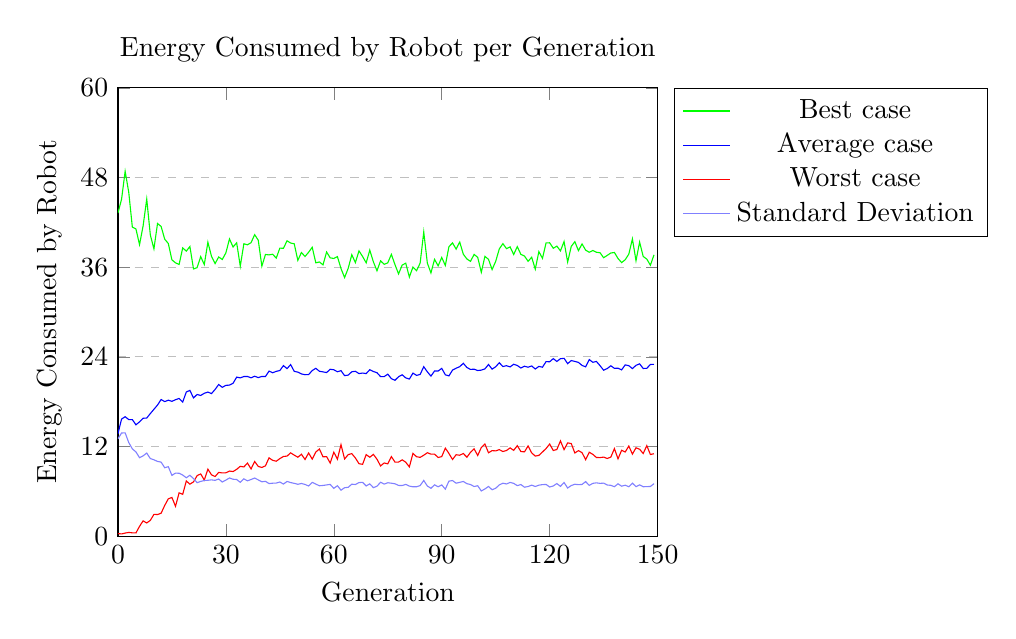
\begin{tikzpicture}
\begin{axis}[
	title={Energy Consumed by Robot per Generation},
	xlabel={Generation},
	ylabel={Energy Consumed by Robot},
	xmin=0, xmax=150,
	ymin=0, ymax=60,
	xtick={0.0,30.0,60.0,90.0,120.0,150.0},
	ytick={0.0,12.0,24.0,36.0,48.0,60.0},
	legend pos=outer north east,
	ymajorgrids=true,
	grid style=dashed,
]

\addplot[
	color=green,
	]
	coordinates {
	(0,43.25)(1,45.083333333333336)(2,48.83333333333335)(3,46.03333333333334)(4,41.36666666666666)(5,41.11666666666667)(6,39.016666666666666)(7,41.550000000000004)(8,45.11666666666667)(9,40.31666666666667)(10,38.45)(11,41.85)(12,41.45)(13,39.75)(14,39.166666666666664)(15,36.98333333333333)(16,36.58333333333333)(17,36.36666666666666)(18,38.583333333333336)(19,38.15)(20,38.76666666666666)(21,35.76666666666667)(22,35.93333333333334)(23,37.41666666666667)(24,36.349999999999994)(25,39.349999999999994)(26,37.45)(27,36.48333333333333)(28,37.36666666666667)(29,37.03333333333334)(30,37.916666666666664)(31,39.78333333333334)(32,38.7)(33,39.266666666666666)(34,36.13333333333334)(35,39.133333333333326)(36,39.0)(37,39.28333333333334)(38,40.35)(39,39.616666666666674)(40,36.13333333333333)(41,37.699999999999996)(42,37.65)(43,37.73333333333333)(44,37.21666666666666)(45,38.550000000000004)(46,38.533333333333324)(47,39.53333333333333)(48,39.23333333333334)(49,39.13333333333333)(50,36.91666666666666)(51,37.96666666666666)(52,37.43333333333333)(53,38.00000000000001)(54,38.666666666666664)(55,36.58333333333333)(56,36.7)(57,36.31666666666666)(58,38.03333333333334)(59,37.25)(60,37.166666666666664)(61,37.41666666666667)(62,35.81666666666667)(63,34.61666666666667)(64,35.85)(65,37.666666666666664)(66,36.61666666666666)(67,38.18333333333334)(68,37.43333333333334)(69,36.58333333333333)(70,38.283333333333324)(71,36.71666666666667)(72,35.516666666666666)(73,36.85)(74,36.383333333333326)(75,36.583333333333336)(76,37.71666666666666)(77,36.35)(78,35.099999999999994)(79,36.283333333333324)(80,36.53333333333333)(81,34.68333333333333)(82,36.016666666666666)(83,35.53333333333334)(84,36.55000000000001)(85,40.71666666666666)(86,36.550000000000004)(87,35.23333333333333)(88,37.05)(89,36.18333333333334)(90,37.300000000000004)(91,36.233333333333334)(92,38.74999999999999)(93,39.24999999999999)(94,38.416666666666664)(95,39.36666666666666)(96,37.73333333333333)(97,37.1)(98,36.783333333333324)(99,37.71666666666666)(100,37.316666666666656)(101,35.31666666666666)(102,37.45000000000001)(103,37.05)(104,35.68333333333334)(105,36.78333333333333)(106,38.45000000000001)(107,39.15)(108,38.48333333333334)(109,38.71666666666666)(110,37.7)(111,38.74999999999999)(112,37.716666666666676)(113,37.5)(114,36.78333333333334)(115,37.333333333333336)(116,35.73333333333334)(117,38.083333333333336)(118,37.18333333333333)(119,39.25)(120,39.266666666666666)(121,38.533333333333346)(122,38.81666666666666)(123,38.18333333333334)(124,39.43333333333334)(125,36.68333333333334)(126,38.78333333333333)(127,39.41666666666667)(128,38.21666666666666)(129,39.11666666666667)(130,38.283333333333346)(131,38.00000000000001)(132,38.233333333333334)(133,37.99999999999999)(134,37.93333333333334)(135,37.266666666666666)(136,37.58333333333333)(137,37.9)(138,37.96666666666666)(139,37.16666666666667)(140,36.61666666666667)(141,37.0)(142,37.74999999999999)(143,39.78333333333334)(144,36.86666666666667)(145,39.36666666666667)(146,37.43333333333332)(147,37.08333333333332)(148,36.266666666666666)(149,37.65)
	};
	\addlegendentry{Best case}
\addplot[
	color=blue,
	]
	coordinates {
	(0,13.702777777777778)(1,15.670833333333333)(2,15.987500000000002)(3,15.606944444444443)(4,15.60625)(5,14.904861111111112)(6,15.30625)(7,15.784722222222225)(8,15.807638888888889)(9,16.409722222222225)(10,16.98194444444444)(11,17.552083333333336)(12,18.293055555555554)(13,18.010416666666664)(14,18.200000000000006)(15,18.050694444444446)(16,18.263888888888886)(17,18.436805555555555)(18,17.95486111111111)(19,19.290277777777778)(20,19.51875)(21,18.50138888888889)(22,18.96666666666667)(23,18.831944444444442)(24,19.120833333333334)(25,19.286805555555556)(26,19.08402777777778)(27,19.638194444444444)(28,20.29722222222222)(29,19.926388888888887)(30,20.186805555555555)(31,20.217361111111103)(32,20.465277777777775)(33,21.289583333333336)(34,21.18402777777778)(35,21.365277777777777)(36,21.377083333333335)(37,21.192361111111104)(38,21.40902777777778)(39,21.22291666666667)(40,21.378472222222225)(41,21.37013888888889)(42,22.09791666666667)(43,21.87152777777778)(44,22.058333333333326)(45,22.175000000000004)(46,22.830555555555552)(47,22.42430555555556)(48,22.962500000000006)(49,22.059722222222224)(50,21.957638888888887)(51,21.714583333333334)(52,21.6125)(53,21.627083333333335)(54,22.167361111111113)(55,22.463888888888885)(56,22.072222222222223)(57,21.988194444444442)(58,21.89930555555555)(59,22.336805555555554)(60,22.274305555555557)(61,22.006249999999998)(62,22.15763888888889)(63,21.486111111111114)(64,21.55902777777778)(65,22.004166666666666)(66,22.067361111111115)(67,21.762500000000003)(68,21.833333333333332)(69,21.759722222222226)(70,22.28194444444445)(71,22.036805555555553)(72,21.87569444444444)(73,21.354166666666664)(74,21.36319444444445)(75,21.684027777777775)(76,21.082638888888887)(77,20.862499999999994)(78,21.340972222222227)(79,21.60138888888888)(80,21.183333333333337)(81,21.02638888888889)(82,21.827083333333338)(83,21.518055555555563)(84,21.647916666666667)(85,22.684027777777782)(86,21.996527777777775)(87,21.42222222222222)(88,22.109027777777783)(89,22.104166666666664)(90,22.463888888888896)(91,21.59861111111111)(92,21.452083333333334)(93,22.227777777777774)(94,22.484722222222224)(95,22.687500000000004)(96,23.14027777777778)(97,22.568055555555556)(98,22.320138888888888)(99,22.35)(100,22.170138888888886)(101,22.223611111111108)(102,22.390972222222224)(103,22.979166666666664)(104,22.352083333333333)(105,22.680555555555557)(106,23.212500000000006)(107,22.70486111111111)(108,22.821527777777778)(109,22.656944444444445)(110,23.00902777777778)(111,22.84861111111111)(112,22.50347222222222)(113,22.745138888888892)(114,22.614583333333332)(115,22.784027777777776)(116,22.374305555555555)(117,22.72222222222222)(118,22.616666666666667)(119,23.363194444444442)(120,23.34236111111111)(121,23.764583333333334)(122,23.384027777777774)(123,23.75555555555556)(124,23.80277777777778)(125,23.087499999999995)(126,23.505555555555556)(127,23.390277777777776)(128,23.258333333333333)(129,22.853472222222223)(130,22.66388888888889)(131,23.641666666666666)(132,23.27361111111111)(133,23.385416666666668)(134,22.819444444444446)(135,22.214583333333337)(136,22.436111111111114)(137,22.80347222222222)(138,22.46527777777777)(139,22.475694444444446)(140,22.26111111111111)(141,22.92777777777778)(142,22.820138888888895)(143,22.431250000000002)(144,22.865277777777777)(145,23.065277777777776)(146,22.44444444444444)(147,22.46944444444445)(148,22.98333333333333)(149,22.987500000000004)
	};
	\addlegendentry{Average case}
\addplot[
	color=red,
	]
	coordinates {
	(0,0.35)(1,0.3)(2,0.41666666666666663)(3,0.49999999999999994)(4,0.44999999999999996)(5,0.4333333333333333)(6,1.3166666666666667)(7,2.0500000000000003)(8,1.7666666666666668)(9,2.1166666666666667)(10,2.9166666666666665)(11,2.9)(12,3.066666666666667)(13,4.116666666666667)(14,5.0)(15,5.183333333333333)(16,4.0)(17,5.8)(18,5.6)(19,7.383333333333332)(20,6.966666666666667)(21,7.266666666666666)(22,8.100000000000001)(23,8.333333333333332)(24,7.516666666666666)(25,8.966666666666669)(26,8.216666666666667)(27,7.983333333333333)(28,8.533333333333333)(29,8.466666666666667)(30,8.483333333333334)(31,8.716666666666667)(32,8.649999999999999)(33,8.950000000000001)(34,9.349999999999998)(35,9.266666666666666)(36,9.783333333333333)(37,9.0)(38,10.0)(39,9.333333333333334)(40,9.2)(41,9.416666666666668)(42,10.483333333333334)(43,10.150000000000002)(44,10.033333333333331)(45,10.38333333333333)(46,10.666666666666668)(47,10.716666666666665)(48,11.149999999999999)(49,10.850000000000001)(50,10.566666666666668)(51,10.966666666666665)(52,10.266666666666666)(53,11.133333333333335)(54,10.316666666666665)(55,11.266666666666667)(56,11.666666666666666)(57,10.616666666666665)(58,10.65)(59,9.783333333333335)(60,11.250000000000002)(61,10.3)(62,12.25)(63,10.333333333333334)(64,10.916666666666664)(65,11.05)(66,10.466666666666669)(67,9.7)(68,9.616666666666667)(69,10.916666666666666)(70,10.566666666666666)(71,10.95)(72,10.300000000000002)(73,9.399999999999999)(74,9.8)(75,9.683333333333332)(76,10.65)(77,9.916666666666666)(78,9.916666666666668)(79,10.216666666666665)(80,9.9)(81,9.266666666666666)(82,11.083333333333334)(83,10.633333333333335)(84,10.549999999999997)(85,10.833333333333334)(86,11.166666666666668)(87,10.983333333333334)(88,10.983333333333333)(89,10.533333333333335)(90,10.65)(91,11.783333333333333)(92,11.066666666666666)(93,10.266666666666667)(94,10.9)(95,10.833333333333332)(96,11.066666666666665)(97,10.566666666666665)(98,11.233333333333333)(99,11.683333333333334)(100,10.8)(101,11.866666666666667)(102,12.333333333333332)(103,11.166666666666663)(104,11.450000000000001)(105,11.416666666666666)(106,11.583333333333334)(107,11.333333333333332)(108,11.466666666666669)(109,11.816666666666666)(110,11.483333333333334)(111,12.116666666666669)(112,11.333333333333334)(113,11.283333333333335)(114,12.083333333333334)(115,11.150000000000002)(116,10.716666666666667)(117,10.816666666666668)(118,11.266666666666667)(119,11.733333333333333)(120,12.333333333333334)(121,11.46666666666667)(122,11.6)(123,12.75)(124,11.583333333333332)(125,12.483333333333333)(126,12.4)(127,11.133333333333331)(128,11.45)(129,11.183333333333332)(130,10.233333333333334)(131,11.233333333333334)(132,10.95)(133,10.533333333333331)(134,10.516666666666667)(135,10.583333333333334)(136,10.399999999999999)(137,10.583333333333332)(138,11.716666666666667)(139,10.35)(140,11.5)(141,11.266666666666664)(142,12.066666666666668)(143,10.983333333333334)(144,11.833333333333334)(145,11.633333333333335)(146,11.066666666666665)(147,12.116666666666669)(148,10.933333333333332)(149,11.033333333333335)
	};
	\addlegendentry{Worst case}
\addplot[
	color=blue!50,
	]
	coordinates {
	(0,13.025428908389014)(1,13.810346550954476)(2,13.828080440847092)(3,12.536856175323127)(4,11.687336506557788)(5,11.278266565587925)(6,10.501986791555993)(7,10.756807752498277)(8,11.123641785695767)(9,10.386590504187978)(10,10.221378626796373)(11,10.0072642842455)(12,9.910259443748078)(13,9.159101324569477)(14,9.303068720464928)(15,8.136114284424643)(16,8.442985588951556)(17,8.419964631951537)(18,8.175106742249568)(19,7.819965516568136)(20,8.152075255391479)(21,7.7114696165346075)(22,7.163779102298379)(23,7.328275304469596)(24,7.4528129284425715)(25,7.481462069336689)(26,7.53842600557016)(27,7.473568842213835)(28,7.652880221410522)(29,7.24745306007676)(30,7.507851449040219)(31,7.789290167969191)(32,7.622416740108644)(33,7.579573710866637)(34,7.209173054431467)(35,7.674179762512963)(36,7.404567722923065)(37,7.587610754448604)(38,7.777959745378355)(39,7.534920928418523)(40,7.276515574031566)(41,7.342139720134329)(42,7.041825948290563)(43,7.090418939649814)(44,7.110711609579553)(45,7.249430618270159)(46,6.97307712015094)(47,7.326380735304754)(48,7.175603845053802)(49,7.071456064751343)(50,6.944892436659276)(51,7.054153593681907)(52,6.925574599185686)(53,6.71816819439981)(54,7.2027313196276594)(55,6.969585256429113)(56,6.747240707808752)(57,6.789921258148179)(58,6.860547540788126)(59,6.928211569219866)(60,6.397805765611721)(61,6.7552421370725675)(62,6.154926673906596)(63,6.485800688397053)(64,6.541500249927993)(65,6.9578287440314055)(66,6.916514655024321)(67,7.171383562116569)(68,7.208015117309649)(69,6.719545525884519)(70,7.0064607939101995)(71,6.492097867347669)(72,6.682439569654588)(73,7.222453389940815)(74,6.969889252912186)(75,7.15245677645985)(76,7.0899056889959375)(77,7.014635159627206)(78,6.791903957601484)(79,6.780344653994618)(80,6.931501668919507)(81,6.7026144154052005)(82,6.6093845948443715)(83,6.6114720266694675)(84,6.776284790786758)(85,7.458544733301797)(86,6.715603927290007)(87,6.40997058389649)(88,6.875571233475309)(89,6.607686022952553)(90,6.861778369888345)(91,6.296488869387335)(92,7.369711299557141)(93,7.444854372659652)(94,7.089891736321568)(95,7.2078004568368925)(96,7.320265729199365)(97,7.027339192380647)(98,6.912254402661862)(99,6.649402026643729)(100,6.748778337282881)(101,6.047367568958867)(102,6.323465498320564)(103,6.651838777617148)(104,6.211944896853704)(105,6.417052304513479)(106,6.860288720300009)(107,7.08864869544486)(108,6.987562242631174)(109,7.195008862591659)(110,7.067679970742447)(111,6.764544671818376)(112,6.910756018467242)(113,6.5563145115801875)(114,6.646507909579263)(115,6.832896938087492)(116,6.650187882020349)(117,6.825224031089765)(118,6.902161583494312)(119,6.925290955648311)(120,6.580437646884687)(121,6.718299856719031)(122,7.040225022091886)(123,6.66810757240103)(124,7.1883639796633565)(125,6.445244453108852)(126,6.7778886188033365)(127,6.948772922857561)(128,6.895431573334017)(129,6.9246965479096385)(130,7.303813108654388)(131,6.797754897530904)(132,7.0714504518847106)(133,7.141901757424131)(134,7.064649642995899)(135,7.101780349676218)(136,6.850000503981754)(137,6.8067826374503815)(138,6.6211205492311365)(139,7.014587725641828)(140,6.69178681032594)(141,6.8212860961759905)(142,6.6210763034866185)(143,7.093520058043778)(144,6.6268579715702)(145,6.870033969272324)(146,6.6170758597207495)(147,6.633982989863595)(148,6.652876244562766)(149,7.028843944036023)
	};
	\addlegendentry{Standard Deviation}
\end{axis}
\end{tikzpicture}
}
		\caption{Some sample caption}
	\end{subfigure}%
	\begin{subfigure}[b]{0.7\textwidth}
		\centering
		\resizebox{0.9\linewidth}{!}{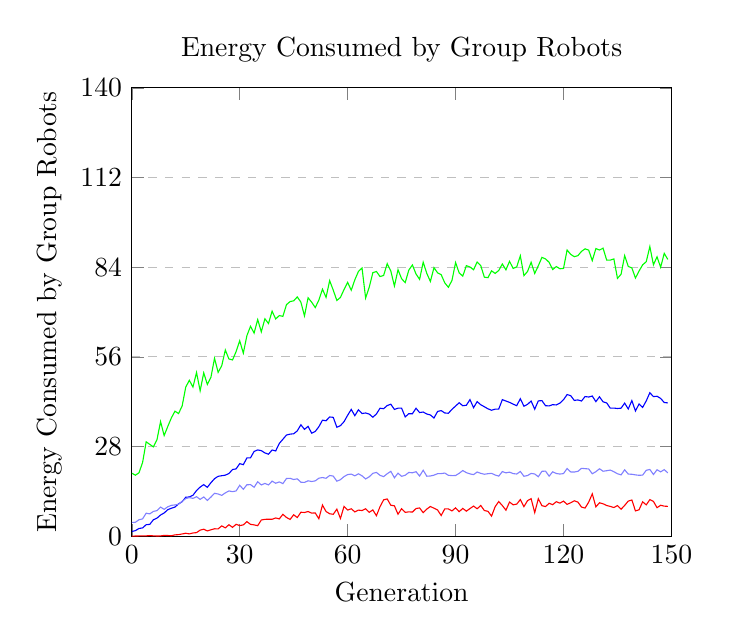
\begin{tikzpicture}
\begin{axis}[
	title={Energy Consumed by Group Robots},
	xlabel={Generation},
	ylabel={Energy Consumed by Group Robots},
	xmin=0, xmax=150,
	ymin=0, ymax=140,
	xtick={0.0,30.0,60.0,90.0,120.0,150.0},
	ytick={0.0,28.0,56.0,84.0,112.0,140.0},
	ymajorgrids=true,
	grid style=dashed,
]

\addplot[
	color=green,
	]
	coordinates {
	(0,19.68333333333333)(1,19.05)(2,19.800000000000004)(3,23.0)(4,29.46666666666666)(5,28.66666666666666)(6,27.900000000000006)(7,30.116666666666656)(8,35.78333333333334)(9,31.416666666666664)(10,34.266666666666666)(11,36.93333333333333)(12,39.03333333333334)(13,38.3)(14,40.666666666666664)(15,46.56666666666666)(16,48.68333333333334)(17,46.56666666666666)(18,51.116666666666674)(19,45.383333333333326)(20,50.99999999999999)(21,47.38333333333333)(22,49.616666666666674)(23,55.56666666666666)(24,51.16666666666666)(25,53.21666666666667)(26,58.15)(27,55.349999999999994)(28,55.03333333333333)(29,57.63333333333333)(30,61.01666666666666)(31,57.166666666666664)(32,62.63333333333335)(33,65.55)(34,63.43333333333332)(35,67.64999999999999)(36,63.81666666666668)(37,67.9)(38,66.41666666666667)(39,70.28333333333332)(40,67.83333333333331)(41,68.89999999999999)(42,68.65000000000002)(43,72.30000000000001)(44,73.26666666666668)(45,73.5)(46,74.71666666666665)(47,73.1)(48,68.8)(49,74.45)(50,73.08333333333334)(51,71.38333333333333)(52,73.73333333333333)(53,77.14999999999999)(54,74.56666666666665)(55,79.8)(56,76.83333333333333)(57,73.61666666666665)(58,74.56666666666669)(59,77.05000000000001)(60,79.24999999999999)(61,76.81666666666669)(62,80.06666666666666)(63,82.68333333333334)(64,83.75)(65,74.36666666666667)(66,77.73333333333333)(67,82.28333333333336)(68,82.64999999999999)(69,81.08333333333331)(70,81.41666666666666)(71,85.1)(72,82.81666666666668)(73,78.13333333333334)(74,83.19999999999999)(75,80.4)(76,79.18333333333335)(77,83.1)(78,84.69999999999999)(79,81.9)(80,80.19999999999999)(81,85.56666666666666)(82,82.06666666666668)(83,79.55000000000001)(84,83.86666666666666)(85,82.25)(86,81.66666666666666)(87,79.11666666666667)(88,77.73333333333332)(89,79.86666666666667)(90,85.46666666666667)(91,82.21666666666664)(92,81.21666666666665)(93,84.48333333333332)(94,84.06666666666668)(95,83.20000000000002)(96,85.63333333333334)(97,84.5)(98,80.88333333333333)(99,80.73333333333333)(100,82.86666666666669)(101,82.06666666666666)(102,82.96666666666667)(103,84.99999999999999)(104,83.18333333333335)(105,85.83333333333333)(106,83.60000000000001)(107,84.10000000000001)(108,87.56666666666666)(109,81.36666666666665)(110,82.66666666666666)(111,85.53333333333333)(112,82.05)(113,84.45)(114,87.06666666666666)(115,86.60000000000001)(116,85.53333333333332)(117,83.26666666666667)(118,84.20000000000002)(119,83.51666666666668)(120,83.61666666666669)(121,89.36666666666666)(122,88.01666666666668)(123,87.28333333333332)(124,87.60000000000002)(125,88.93333333333332)(126,89.73333333333335)(127,89.33333333333334)(128,86.04999999999998)(129,89.81666666666668)(130,89.36666666666667)(131,89.93333333333335)(132,86.23333333333333)(133,86.2)(134,86.58333333333333)(135,80.51666666666665)(136,81.78333333333332)(137,87.6)(138,84.23333333333333)(139,83.78333333333335)(140,80.61666666666666)(141,82.79999999999998)(142,84.73333333333335)(143,85.71666666666665)(144,90.45000000000002)(145,84.75)(146,87.25000000000001)(147,83.96666666666667)(148,88.31666666666668)(149,86.43333333333332)
	};
\addplot[
	color=blue,
	]
	coordinates {
	(0,1.4493055555555556)(1,1.7402777777777778)(2,2.4076388888888887)(3,2.5819444444444444)(4,3.5854166666666667)(5,3.692361111111111)(6,5.127083333333332)(7,5.63888888888889)(8,6.620833333333333)(9,7.252083333333332)(10,8.265277777777778)(11,8.738194444444446)(12,9.101388888888888)(13,10.08125)(14,10.765277777777778)(15,12.162500000000001)(16,12.256944444444445)(17,12.770138888888889)(18,14.259027777777774)(19,15.331944444444442)(20,16.100694444444443)(21,15.260416666666666)(22,16.70486111111111)(23,17.95277777777778)(24,18.69236111111111)(25,18.883333333333333)(26,19.063194444444438)(27,19.570833333333336)(28,20.820833333333333)(29,21.018749999999997)(30,22.664583333333333)(31,22.329166666666666)(32,24.445138888888888)(33,24.46944444444445)(34,26.471527777777776)(35,26.93125)(36,26.719444444444445)(37,26.008333333333336)(38,25.60138888888889)(39,26.923611111111104)(40,26.626388888888886)(41,28.961111111111112)(42,30.273611111111112)(43,31.591666666666665)(44,31.87291666666666)(45,31.984027777777783)(46,32.88680555555555)(47,34.790972222222216)(48,33.365972222222226)(49,34.29722222222222)(50,32.173611111111114)(51,32.70416666666667)(52,34.19375000000001)(53,36.235416666666666)(54,36.04999999999998)(55,37.226388888888884)(56,37.118055555555564)(57,34.013888888888886)(58,34.52291666666666)(59,35.77222222222222)(60,37.755555555555546)(61,39.6)(62,37.637499999999996)(63,39.48680555555555)(64,38.30902777777777)(65,38.47777777777779)(66,38.13472222222222)(67,37.14652777777777)(68,38.172916666666666)(69,39.96319444444444)(70,39.813194444444456)(71,40.79583333333333)(72,41.215277777777764)(73,39.584722222222226)(74,39.97083333333333)(75,39.97291666666667)(76,37.25277777777777)(77,38.25694444444444)(78,38.22916666666667)(79,39.95069444444446)(80,38.60902777777778)(81,38.77500000000001)(82,38.153472222222234)(83,37.86805555555555)(84,36.900000000000006)(85,38.956944444444446)(86,39.21875000000001)(87,38.48125)(88,38.39236111111112)(89,39.615277777777784)(90,40.64166666666667)(91,41.67569444444444)(92,40.74166666666667)(93,40.892361111111114)(94,42.648611111111116)(95,40.12430555555556)(96,42.02708333333332)(97,41.047222222222224)(98,40.42430555555555)(99,39.772916666666674)(100,39.331250000000004)(101,39.672222222222224)(102,39.71041666666666)(103,42.641666666666666)(104,42.20625)(105,41.793749999999996)(106,41.233333333333334)(107,40.75902777777778)(108,42.93958333333333)(109,40.58958333333332)(110,41.170833333333334)(111,42.202083333333334)(112,39.6625)(113,42.25486111111111)(114,42.334722222222226)(115,40.75000000000001)(116,40.68750000000001)(117,41.072222222222216)(118,40.97986111111111)(119,41.560416666666676)(120,42.61736111111111)(121,44.22569444444444)(122,43.88333333333333)(123,42.394444444444446)(124,42.55694444444443)(125,42.211111111111116)(126,43.6076388888889)(127,43.4625)(128,43.76666666666666)(129,42.02361111111111)(130,43.53611111111112)(131,41.96041666666667)(132,41.624305555555544)(133,39.97430555555556)(134,40.00555555555555)(135,39.87569444444444)(136,39.97708333333334)(137,41.54930555555555)(138,39.72638888888888)(139,42.34652777777777)(140,39.09097222222223)(141,41.294444444444444)(142,40.22361111111111)(143,42.24513888888889)(144,44.80277777777777)(145,43.58333333333333)(146,43.69930555555556)(147,43.02430555555556)(148,41.73888888888888)(149,41.625)
	};
\addplot[
	color=red,
	]
	coordinates {
	(0,0.016666666666666666)(1,0.05)(2,0.08333333333333333)(3,0.08333333333333333)(4,0.09999999999999999)(5,0.19999999999999998)(6,0.09999999999999999)(7,0.06666666666666667)(8,0.08333333333333334)(9,0.25)(10,0.21666666666666667)(11,0.13333333333333333)(12,0.41666666666666663)(13,0.4833333333333333)(14,0.7)(15,0.9166666666666666)(16,0.7166666666666667)(17,1.0000000000000002)(18,1.1166666666666667)(19,1.9000000000000001)(20,2.183333333333333)(21,1.6499999999999997)(22,2.0)(23,2.316666666666667)(24,2.283333333333333)(25,3.2166666666666663)(26,2.6)(27,3.5833333333333335)(28,2.7666666666666666)(29,3.7166666666666663)(30,3.3000000000000003)(31,3.5333333333333337)(32,4.55)(33,3.6999999999999993)(34,3.5333333333333328)(35,3.2833333333333328)(36,5.05)(37,5.266666666666667)(38,5.299999999999999)(39,5.283333333333333)(40,5.699999999999999)(41,5.4)(42,6.833333333333334)(43,5.85)(44,5.233333333333333)(45,6.683333333333334)(46,5.816666666666667)(47,7.4833333333333325)(48,7.400000000000002)(49,7.699999999999999)(50,7.216666666666667)(51,7.250000000000001)(52,5.449999999999998)(53,9.733333333333333)(54,7.7)(55,7.0166666666666675)(56,6.833333333333332)(57,8.450000000000001)(58,5.533333333333332)(59,9.316666666666665)(60,8.149999999999999)(61,8.566666666666668)(62,7.6)(63,8.149999999999999)(64,8.0)(65,8.583333333333332)(66,7.449999999999999)(67,8.2)(68,6.3999999999999995)(69,9.216666666666665)(70,11.35)(71,11.633333333333333)(72,9.666666666666666)(73,9.483333333333334)(74,6.866666666666666)(75,8.6)(76,7.450000000000001)(77,7.600000000000001)(78,7.533333333333333)(79,8.633333333333335)(80,8.816666666666668)(81,7.35)(82,8.466666666666665)(83,9.283333333333335)(84,8.733333333333333)(85,8.183333333333334)(86,6.466666666666667)(87,8.549999999999999)(88,8.516666666666666)(89,7.9)(90,8.850000000000001)(91,7.649999999999999)(92,8.683333333333334)(93,7.8166666666666655)(94,8.633333333333336)(95,9.4)(96,8.566666666666668)(97,9.583333333333334)(98,8.016666666666667)(99,7.766666666666666)(100,6.266666666666666)(101,9.216666666666665)(102,10.816666666666668)(103,9.566666666666665)(104,8.116666666666667)(105,10.666666666666668)(106,9.799999999999999)(107,10.016666666666666)(108,11.433333333333334)(109,9.233333333333333)(110,11.1)(111,11.716666666666669)(112,7.366666666666666)(113,11.7)(114,9.533333333333333)(115,9.250000000000002)(116,10.266666666666666)(117,9.85)(118,10.766666666666666)(119,10.333333333333334)(120,10.950000000000001)(121,9.95)(122,10.433333333333334)(123,11.05)(124,10.65)(125,9.1)(126,8.783333333333335)(127,10.633333333333335)(128,13.216666666666669)(129,9.166666666666664)(130,10.433333333333334)(131,10.116666666666667)(132,9.583333333333332)(133,9.299999999999999)(134,8.95)(135,9.566666666666666)(136,8.416666666666668)(137,9.616666666666667)(138,10.966666666666665)(139,11.3)(140,7.8999999999999995)(141,8.25)(142,10.733333333333333)(143,9.783333333333333)(144,11.416666666666666)(145,10.85)(146,8.899999999999999)(147,9.666666666666668)(148,9.383333333333335)(149,9.316666666666668)
	};
\addplot[
	color=blue!50,
	]
	coordinates {
	(0,4.28643110259652)(1,4.350004465706617)(2,5.1353585814671305)(3,5.4036342055382836)(4,7.184036432091683)(5,6.959859072520352)(6,7.740183076680505)(7,7.9895584403415265)(8,9.095487652655299)(9,8.382295176141476)(10,9.175423944208907)(11,9.633879288381019)(12,9.768514050354678)(13,9.974388115867566)(14,10.894458482255986)(15,11.738536762885685)(16,12.052917874791023)(17,11.809426929647783)(18,12.327754549882282)(19,11.491843569692882)(20,12.24759609905034)(21,11.17672592269558)(22,12.219402932220374)(23,13.39188482037835)(24,13.177696287681739)(25,12.74766297624472)(26,13.521821381657194)(27,14.135044010423613)(28,13.906055403578163)(29,14.128742493983314)(30,15.902322644410466)(31,14.645396418128552)(32,16.060336930196915)(33,16.099668682455683)(34,15.28406147186754)(35,16.99790090836383)(36,15.996187485351106)(37,16.48239954714082)(38,16.016387608916656)(39,17.18999929190662)(40,16.538603152238476)(41,16.947777823923516)(42,16.424612841552417)(43,18.01001504802194)(44,18.078239704517717)(45,17.704079890445904)(46,17.913934301523216)(47,16.852624241279187)(48,16.790068127011928)(49,17.295830669086403)(50,17.078290689305945)(51,17.275993085175653)(52,18.117950075812907)(53,18.311959715112405)(54,18.08517279742271)(55,18.953098229289978)(56,18.767837639776488)(57,17.172012659257902)(58,17.65097508376289)(59,18.62404914701312)(60,19.238944827068806)(61,19.392432617191513)(62,18.845586300539566)(63,19.48640298916557)(64,18.858058411573936)(65,17.878337930467147)(66,18.55605846283305)(67,19.63556833827702)(68,19.915277309552184)(69,19.006921915917616)(70,18.597254446813317)(71,19.509070380318636)(72,20.262762845648705)(73,18.2368857544476)(74,19.674839801461772)(75,18.69521328303294)(76,19.030233509955085)(77,19.907718252012586)(78,19.79814700277209)(79,20.137561765560616)(80,18.795355068425618)(81,20.59535530390388)(82,18.72987040604221)(83,18.798325829024964)(84,19.060857959296605)(85,19.51787743213442)(86,19.54489190339996)(87,19.711786355157944)(88,19.009380833146565)(89,18.927774516737333)(90,18.947015282128955)(91,19.638613342366703)(92,20.49930164229917)(93,19.853511291764768)(94,19.459606929036465)(95,19.23188996151202)(96,20.038325925091844)(97,19.61997688067101)(98,19.3507354587123)(99,19.514163896455432)(100,19.631598058091992)(101,19.109664015582222)(102,18.756192501638573)(103,20.180840343035893)(104,19.773228850286245)(105,20.002454347760107)(106,19.54912126207232)(107,19.418074851634312)(108,20.206758169014982)(109,18.710740906744913)(110,18.93617145351968)(111,19.61620260966329)(112,19.423176715801702)(113,18.560247256359798)(114,20.25783868884567)(115,20.325005765811206)(116,18.75070538397598)(117,20.099168440707494)(118,19.587735379855705)(119,19.40600950617213)(120,19.551509454546206)(121,21.13214833612396)(122,20.06398796601037)(123,20.037555187318954)(124,20.250837917539858)(125,21.193432242675417)(126,21.09177383269476)(127,20.992179395339345)(128,19.496413740982774)(129,20.14352512409504)(130,21.052582318385543)(131,20.286633139465597)(132,20.450394077134284)(133,20.64914510944557)(134,20.137723555109858)(135,19.499307880893333)(136,19.146987961702894)(137,20.7307583172003)(138,19.39964134770471)(139,19.335344872430053)(140,19.146794263155318)(141,19.01098423522314)(142,19.07965716709215)(143,20.57695874353471)(144,20.839029859801943)(145,19.26633036046936)(146,20.748815778140724)(147,20.091755087016924)(148,20.79314639778314)(149,19.767443043138652)
	};
\end{axis}
\end{tikzpicture}
}
		\caption{Some sample caption}
	\end{subfigure}%
}
\end{figure}
